% =====================================================================
%  Computational Details -- Supporting Information section
%  "Surface Oxidation State Controls Product Selectivity in Autothermal
%   Reforming of Ammonia over Ru Catalysts"
%
%  USAGE (Overleaf): put  % =====================================================================
%  Computational Details -- Supporting Information section
%  "Surface Oxidation State Controls Product Selectivity in Autothermal
%   Reforming of Ammonia over Ru Catalysts"
%
%  USAGE (Overleaf): put  % =====================================================================
%  Computational Details -- Supporting Information section
%  "Surface Oxidation State Controls Product Selectivity in Autothermal
%   Reforming of Ammonia over Ru Catalysts"
%
%  USAGE (Overleaf): put  % =====================================================================
%  Computational Details -- Supporting Information section
%  "Surface Oxidation State Controls Product Selectivity in Autothermal
%   Reforming of Ammonia over Ru Catalysts"
%
%  USAGE (Overleaf): put  \input{computational_details}  where this section
%  should appear (e.g. in the Supporting Information). Requires amsmath +
%  amssymb, which are already loaded in ATR NH3.tex.
%
%  FIGURE: the bulk-referenced grand-potential figure uses graphicx (already
%  loaded in ATR NH3.tex) and the image file fig_bulk_referenced_2x2_dft.png,
%  which is committed alongside this .tex at the project root.
%
%  OPTIONAL SI equation numbering (S11, S12, ...): add these two lines to
%  your PREAMBLE, before \begin{document}:
%     \renewcommand{\theequation}{S\arabic{equation}}
%     \setcounter{equation}{10}
%
%  NOTE (revtex twocolumn): the three wide displays (Svib, dOmega/A, log10)
%  can overflow a single column; wrap them in \begin{widetext}...\end{widetext}
%  or compile the SI in onecolumn if they run over.
% =====================================================================

\section*{Computational Details}

\subsection*{Electronic-structure calculations}
Spin-polarized density functional theory (DFT) calculations were performed with
the Perdew--Burke--Ernzerhof (PBE) exchange--correlation functional in the Vienna
\textit{Ab initio} Simulation Package (VASP), using the projector augmented-wave
method and a 430~eV plane-wave cutoff, as detailed in Section~2 of the main text.
The RuO$_2$(110) surfaces were modeled as $(2\times2)$ three-trilayer slabs and
the Ru(0001) surface as a $(4\times4)$ slab, each separated from its periodic
images by a vacuum gap.

\subsection*{Free-energy corrections}
The Gibbs free energy of every slab configuration used in the thermodynamic
analysis is evaluated from its DFT total energy $E_{\mathrm{DFT}}$ together with
the zero-point energy and vibrational (entropic) corrections obtained from the
harmonic vibrational frequencies $\nu_i$:
\begin{equation}
  G_{\mathrm{slab}}(T) = E_{\mathrm{DFT}} + E_{\mathrm{ZPE}}
  - T\,S_{\mathrm{vib}}(T)
  \label{eq:Gslab}
\end{equation}
\begin{equation}
  E_{\mathrm{ZPE}} = \tfrac{1}{2}\sum_i h\nu_i
  \label{eq:ZPE}
\end{equation}
\begin{equation}
  S_{\mathrm{vib}}(T) = k_{\mathrm B}\sum_i\left[
    \frac{h\nu_i/k_{\mathrm B}T}{e^{\,h\nu_i/k_{\mathrm B}T}-1}
    - \ln\!\left(1-e^{-h\nu_i/k_{\mathrm B}T}\right)\right]
  \label{eq:Svib}
\end{equation}
where $k_{\mathrm B}$ and $h$ are the Boltzmann and Planck constants. Because the
zero-point and vibrational-entropy terms are folded directly into
$G_{\mathrm{slab}}(T)$, the tabulated slab free energies are temperature
dependent (e.g., \textit{o}-RuO$_2$(110) 0v: $-817.70$~eV at $0$~K
$\rightarrow -837.48$~eV at $1200$~K), and no additional entropy term is applied
in the grand-potential expressions below. Vibrational frequencies of gas-phase
species were taken from the NIST Computational Chemistry Comparison and Benchmark
Database.

\subsection*{Oxygen reservoir chemical potential}
The surface exchanges lattice oxygen with a gas-phase O$_2$ reservoir. At
temperature $T$ and pressure $p$ the reservoir chemical potential varies with
pressure as
\begin{equation}
  \mu_{\mathrm{O_2}}(T,p) = \mu_{\mathrm{O_2}}(T,p^{0})
  + k_{\mathrm B}T\ln\!\left(p/p^{0}\right)
  \label{eq:muO2}
\end{equation}
and the oxygen chemical potential is one-half of it, referenced to the $0$~K DFT
O$_2$ energy:
\begin{equation}
  \mu_{\mathrm O}(T,p) = \tfrac{1}{2}\mu_{\mathrm{O_2}}(T,p)
  = \tfrac{1}{2}G_{\mathrm{O_2}}(0\,\mathrm{K}) + \Delta\mu_{\mathrm O}
  \label{eq:muO}
\end{equation}
\begin{equation}
  \Delta\mu_{\mathrm O} =
  \tfrac{1}{2}\left[G_{\mathrm{O_2}}(T) - G_{\mathrm{O_2}}(0\,\mathrm{K})\right]
  + \tfrac{1}{2}k_{\mathrm B}T\ln\!\left(p_{\mathrm{O_2}}/p^{0}\right)
  \label{eq:dmuO}
\end{equation}
so that $\Delta\mu_{\mathrm O}=0$ corresponds to gas-phase O$_2$ at $0$~K and more
negative $\Delta\mu_{\mathrm O}$ denotes more reducing conditions. The thermal term
$\tfrac{1}{2}[G_{\mathrm{O_2}}(T)-G_{\mathrm{O_2}}(0\,\mathrm{K})]$ is evaluated
directly from our calculated ideal-gas Gibbs free energy of O$_2$ (translational,
rotational, and vibrational contributions), giving $-0.23$, $-0.57$, $-0.93$, and
$-1.31$~eV per O atom at $298$, $600$, $900$, and $1200$~K, respectively.

\subsection*{Surface grand potential}
The grand potential of a slab open to the oxygen reservoir is
\begin{equation}
  \Omega = U - T\,S(T) - \sum_i \mu_i N_i
  \label{eq:Omega_gen}
\end{equation}
Using the slab free energy of Eq.~\eqref{eq:Gslab} for the $U-TS$ term and noting
that only oxygen is exchanged with the reservoir while ruthenium is conserved,
this becomes
\begin{equation}
  \Omega = G_{\mathrm{slab}}(T) - \mu_{\mathrm O} N_{\mathrm O}
  - \mu_{\mathrm{Ru}} N_{\mathrm{Ru}}
  \label{eq:Omega_surf}
\end{equation}
where $N_{\mathrm O}$ and $N_{\mathrm{Ru}}$ are the numbers of O and Ru atoms in
the cell. Because every termination contains the same $N_{\mathrm{Ru}}=36$, the
$\mu_{\mathrm{Ru}}N_{\mathrm{Ru}}$ term is identical across surfaces and cancels
when grand potentials are compared.

\subsection*{Relative (referenced) grand potential}
Terminations are compared through the grand potential of each $k$-vacancy surface
relative to a vacancy-free reference, per unit surface area $A$
($=119.70~\text{\AA}^{2}$ for the $(2\times2)$ cell):
\begin{equation}
  \frac{\Delta\Omega_k}{A} =
  \frac{\left[G_{\mathrm{slab}}^{(k)}(T)
  - G_{\mathrm{slab}}^{(\mathrm{ref})}(T)\right]
  + n_{\mathrm{vac}}\left(\tfrac{1}{2}G_{\mathrm{O_2}}(0\,\mathrm{K})
  + \Delta\mu_{\mathrm O}\right)}{A}
  \label{eq:dOmega}
\end{equation}
where $n_{\mathrm{vac}} = N_{\mathrm O}^{(\mathrm{ref})} - N_{\mathrm O}^{(k)}$ is
the number of oxygen atoms removed relative to the reference, so the slope of each
line, $n_{\mathrm{vac}}/A$, is the areal density of released oxygen. The
referencing subtracts a common term ($\mu_{\mathrm{Ru}}N_{\mathrm{Ru}}$ and the
bulk contribution), making $\Delta\Omega$ independent of the ruthenium reference.
This relative construction is thermodynamically equivalent to the absolute surface
free energy $\gamma = (1/A)[\,G_{\mathrm{slab}} - N_{\mathrm{Ru}}\,g^{\mathrm{bulk}}_{\mathrm{RuO_2}}
- (N_{\mathrm O}-2N_{\mathrm{Ru}})\,\mu_{\mathrm O}\,]$ of Reuter and Scheffler
[K.~Reuter and M.~Scheffler, Phys.\ Rev.\ B \textbf{65}, 035406 (2001)]: because
every termination shares the same $N_{\mathrm{Ru}}$, referencing to the
\textit{o}-RuO$_2$(110) 0v surface removes the $\mu_{\mathrm{Ru}}$ term by
construction, instead of through the bulk-equilibrium constraint
$\mu_{\mathrm{Ru}}+2\mu_{\mathrm O}=g^{\mathrm{bulk}}_{\mathrm{RuO_2}}$ that references
$\gamma$ to bulk RuO$_2$; both choices leave every crossover and vacancy-formation
threshold unchanged.
This unified construction is shown in Figure~\ref{fig:unified}, in which all
terminations share the single \textit{o}-RuO$_2$(110) 0v reference, using the fact
that \textit{s}-RuO$_2$(110) 0v is \textit{o}-RuO$_2$(110) with its six on-top
oxygens removed (Ru$_{36}$O$_{78} \rightarrow$ Ru$_{36}$O$_{72}$,
$n_{\mathrm{vac}}=6$). The equivalent diagram referenced to bulk RuO$_2$ is shown
in Figure~\ref{fig:bulkref}; presenting the two reference choices side by side
demonstrates that the \textit{o}$\rightarrow$\textit{s} crossover and
vacancy-formation thresholds are independent of the reference.

\subsection*{Operating oxygen chemical potentials}
The ATR inlet is set by a fixed feed oxygen partial pressure
(O$_2$/NH$_3 = 0.25 \rightarrow p_{\mathrm{O_2}} = 0.2$~bar):
\begin{equation}
  \Delta\mu_{\mathrm O}^{\,\mathrm{inlet}} =
  \tfrac{1}{2}\left[G_{\mathrm{O_2}}(T) - G_{\mathrm{O_2}}(0\,\mathrm{K})\right]
  + \tfrac{1}{2}k_{\mathrm B}T\ln\!\left(p_{\mathrm{O_2}}/p^{0}\right)
  \label{eq:inlet}
\end{equation}
The downstream reforming potential is fixed by the
H$_2 + \tfrac{1}{2}$O$_2 \rightleftharpoons$ H$_2$O equilibrium, and is
independent of the O$_2$ reference:
\begin{equation}
  \Delta\mu_{\mathrm O}^{\,\mathrm{down}} =
  \left[G_{\mathrm{H_2O}}(T) - G_{\mathrm{H_2}}(T)\right]
  - \tfrac{1}{2}G_{\mathrm{O_2}}(0\,\mathrm{K})
  + k_{\mathrm B}T\ln\!\left(p_{\mathrm{H_2O}}/p_{\mathrm{H_2}}\right)
  \label{eq:down}
\end{equation}
evaluated at $p_{\mathrm{H_2O}}/p_{\mathrm{H_2}}=10$. The upper axes of
Figures~\ref{fig:unified} and~\ref{fig:bulkref} convert $\Delta\mu_{\mathrm O}$
into an equivalent O$_2$ partial pressure by
inverting Eq.~\eqref{eq:dmuO}:
\begin{equation}
  \log_{10}\!\left(p_{\mathrm{O_2}}/p^{0}\right) =
  \frac{\Delta\mu_{\mathrm O}
  - \tfrac{1}{2}\left(G_{\mathrm{O_2}}(T) - G_{\mathrm{O_2}}(0\,\mathrm{K})\right)}
       {\tfrac{1}{2}k_{\mathrm B}T\ln 10}
  \label{eq:pO2}
\end{equation}
with $p^{0}=1$~bar the standard-state pressure.

\subsection*{Bulk-referenced surface stability and correlation to ATR conditions}
Referencing the surface grand potential to bulk RuO$_2$ rather than to the
\textit{o}-RuO$_2$(110) 0v surface converts the relative curves of
Eq.~\eqref{eq:dOmega} into absolute surface free energies
$\gamma(\Delta\mu_{\mathrm O})$ and, in addition, places the accessible oxygen
chemical potential on a physical scale bounded by two limits. The oxygen-rich
limit is fixed by O$_2$ condensation, $\Delta\mu_{\mathrm O}=0$; the oxygen-poor
limit is fixed by decomposition of the oxide into metallic ruthenium,
$\mathrm{RuO_2}\rightarrow\mathrm{Ru}+\mathrm{O_2}$, which occurs when
\begin{equation}
  \Delta\mu_{\mathrm O}^{\,\mathrm{poor}} =
  \tfrac{1}{2}\,\Delta H_f^{\,\mathrm{RuO_2}} \approx -1.60~\mathrm{eV},
  \label{eq:opoor}
\end{equation}
using the experimental heat of formation $\Delta H_f^{\,\mathrm{RuO_2}}=-3.19$~eV
[NIST--JANAF; consistent with the value adopted by Reuter and Scheffler,
Phys.\ Rev.\ B \textbf{68}, 045407 (2003)]. Because $\Delta\mu_{\mathrm O}$
already carries the full temperature and pressure dependence of the O$_2$
reservoir (Eq.~\eqref{eq:dmuO}), this decomposition bound is temperature
independent. Figure~\ref{fig:bulkref} shows the resulting diagram at 298, 600,
900 and 1200~K. In this reference the stoichiometric \textit{s}-RuO$_2$(110) 0v
surface ($N_{\mathrm O}=2N_{\mathrm{Ru}}$) is flat, whereas every oxygen-rich
termination slopes downward with a slope equal to its excess-oxygen areal
density, $-(N_{\mathrm O}-2N_{\mathrm{Ru}})/A$
($-50.1$~meV\,\AA$^{-2}$\,eV$^{-1}$ for the six on-top oxygens of
\textit{o}-RuO$_2$(110) 0v). Every \textit{o}$\rightarrow$\textit{s} crossover is
numerically identical to that of the \textit{o}-RuO$_2$(110)-referenced diagram
(Figure~\ref{fig:unified}), confirming that the surface phase
boundaries are independent of the chosen reference.

At any oxygen potential the thermodynamically stable surface is simply the
termination of lowest $\gamma$. On the oxygen-rich (right) side of each panel this
is the steeply sloped, oxygen-covered \textit{o}-RuO$_2$(110) surface; on the
oxygen-poor (left) side it is the flat stoichiometric \textit{s}-RuO$_2$(110)
0v surface. The dotted vertical line marks the oxygen potential at which the two are
equally stable---the \textit{o}$\rightarrow$\textit{s} boundary---at
$\Delta\mu_{\mathrm O}=-1.02$, $-1.17$, $-1.36$ and $-1.58$~eV for 298, 600, 900
and 1200~K, respectively. To the right of this line the oxidised
\textit{o}-RuO$_2$(110) surface is stable; to the left, the surface has released its
on-top oxygens to become the reduced \textit{s}-RuO$_2$(110) termination. The closer
an operating point sits to this boundary, the smaller the free-energy margin (a few
meV\,\AA$^{-2}$) between the two terminations, so near it the oxidised and reduced
surfaces are effectively degenerate within DFT accuracy.

Superimposing the ATR operating potentials of
Eqs.~\eqref{eq:inlet}--\eqref{eq:down} on this stability window links the surface
oxidation state directly to reactor position. At the ATR inlet
($\mathrm{O_2/NH_3}=0.25$, $p_{\mathrm{O_2}}=0.2$~bar) the oxygen potential
$\Delta\mu_{\mathrm O}^{\,\mathrm{inlet}}$ ranges from $-0.25$~eV at 298~K to
$-1.39$~eV at 1200~K; it lies inside the RuO$_2$ stability window at every
temperature and on the oxygen-rich side of the
\textit{o}$\rightarrow$\textit{s} crossover, so the inlet surface is the
oxygen-covered \textit{o}-RuO$_2$(110) termination. Downstream, once the
$\mathrm{H_2O/H_2}$ reforming equilibrium is established
($\Delta\mu_{\mathrm O}^{\,\mathrm{down}}\approx-2.3$~eV at
$p_{\mathrm{H_2O}}/p_{\mathrm{H_2}}=10$), the potential falls \emph{below} the
oxide-decomposition bound of Eq.~\eqref{eq:opoor} at all temperatures: the
reducing reforming atmosphere drives the termination through the
\textit{s}-RuO$_2$(110) surface and ultimately toward metallic ruthenium. The
\textit{o}$\rightarrow$\textit{s} crossover ($-1.02$ to $-1.58$~eV) sits between
these two operating points, so a catalyst particle necessarily evolves from the
selective, oxygen-rich \textit{o}-RuO$_2$ surface near the inlet to the reduced
\textit{s}-RuO$_2$ surface as ammonia is consumed and the local gas becomes
reducing. Increasing temperature compresses this window: at 1200~K the inlet
potential ($-1.39$~eV), the \textit{o}$\rightarrow$\textit{s} crossover
($-1.58$~eV) and the decomposition bound ($-1.60$~eV) nearly coincide, so the
reduced surface---and eventually metallic Ru---becomes accessible even close to
the inlet, consistent with the loss of N$_2$ selectivity observed at high
temperature.

Reading these transitions on the equivalent oxygen-pressure scale (upper axes of
Figure~\ref{fig:bulkref}, Eq.~\eqref{eq:pO2}) makes the reactor gradient
explicit. Table~\ref{tab:po2markers} lists the oxygen partial pressure
$p_{\mathrm{O_2}}$ at the inlet, at the \textit{o}$\rightarrow$\textit{s}
crossover, at the oxide-decomposition bound and at the downstream reforming
point. As O$_2$ is consumed along the bed the local oxygen potential sweeps
monotonically toward lower $p_{\mathrm{O_2}}$, so a catalyst particle crosses
these markers in sequence: the oxygen-covered \textit{o}-RuO$_2$(110)
termination at the inlet, the \textit{o}$\rightarrow$\textit{s} transition once
$p_{\mathrm{O_2}}$ has dropped by the margin listed in the final column, and
finally reduction past the decomposition bound in the reforming zone. This
oxidative margin collapses from $\sim$26 orders of magnitude in
$p_{\mathrm{O_2}}$ at 298~K to only $\sim$1.7 at 1200~K, where the crossover and
the decomposition bound become numerically coincident
($p_{\mathrm{O_2}}\approx10^{-2.4}$~bar). The oxygen-covered, N$_2$-selective
surface therefore persists over essentially the entire bed at low temperature
but is confined to a thin zone near the inlet at high temperature, providing a
thermodynamic rationale for the loss of N$_2$ selectivity as temperature
increases.

\begin{table*}[htbp]
  \centering
  \caption{Equivalent oxygen partial pressure $p_{\mathrm{O_2}}$ (bar) at the
  ATR inlet, the \textit{o}$\rightarrow$\textit{s} crossover, the oxygen-poor
  (decomposition) bound and the downstream reforming point, obtained from the
  operating potentials (Eqs.~\eqref{eq:inlet}--\eqref{eq:down}) through
  Eq.~\eqref{eq:pO2}. The final column is the oxidative margin: the drop in
  $p_{\mathrm{O_2}}$ (orders of magnitude) between the inlet and the
  \textit{o}$\rightarrow$\textit{s} crossover.}
  \label{tab:po2markers}
  \begin{tabular}{cccccc}
    \hline
    $T$ (K) & inlet & \textit{o}$\rightarrow$\textit{s} &
    O-poor ($\rightarrow$Ru) & downstream &
    inlet$\rightarrow$\,\textit{o}$\rightarrow$\textit{s} \\
     & (bar) & (bar) & (bar) & (bar) & (decades) \\
    \hline
    298  & $0.2$ & $10^{-27}$  & $10^{-46}$  & $10^{-69}$  & 26  \\
    600  & $0.2$ & $10^{-10}$  & $10^{-17}$  & $10^{-29}$  & 9.5 \\
    900  & $0.2$ & $10^{-4.9}$ & $10^{-7.5}$ & $10^{-16}$  & 4.2 \\
    1200 & $0.2$ & $10^{-2.4}$ & $10^{-2.4}$ & $10^{-9.1}$ & 1.7 \\
    \hline
  \end{tabular}
\end{table*}

\begin{figure*}[htbp]
  \centering
  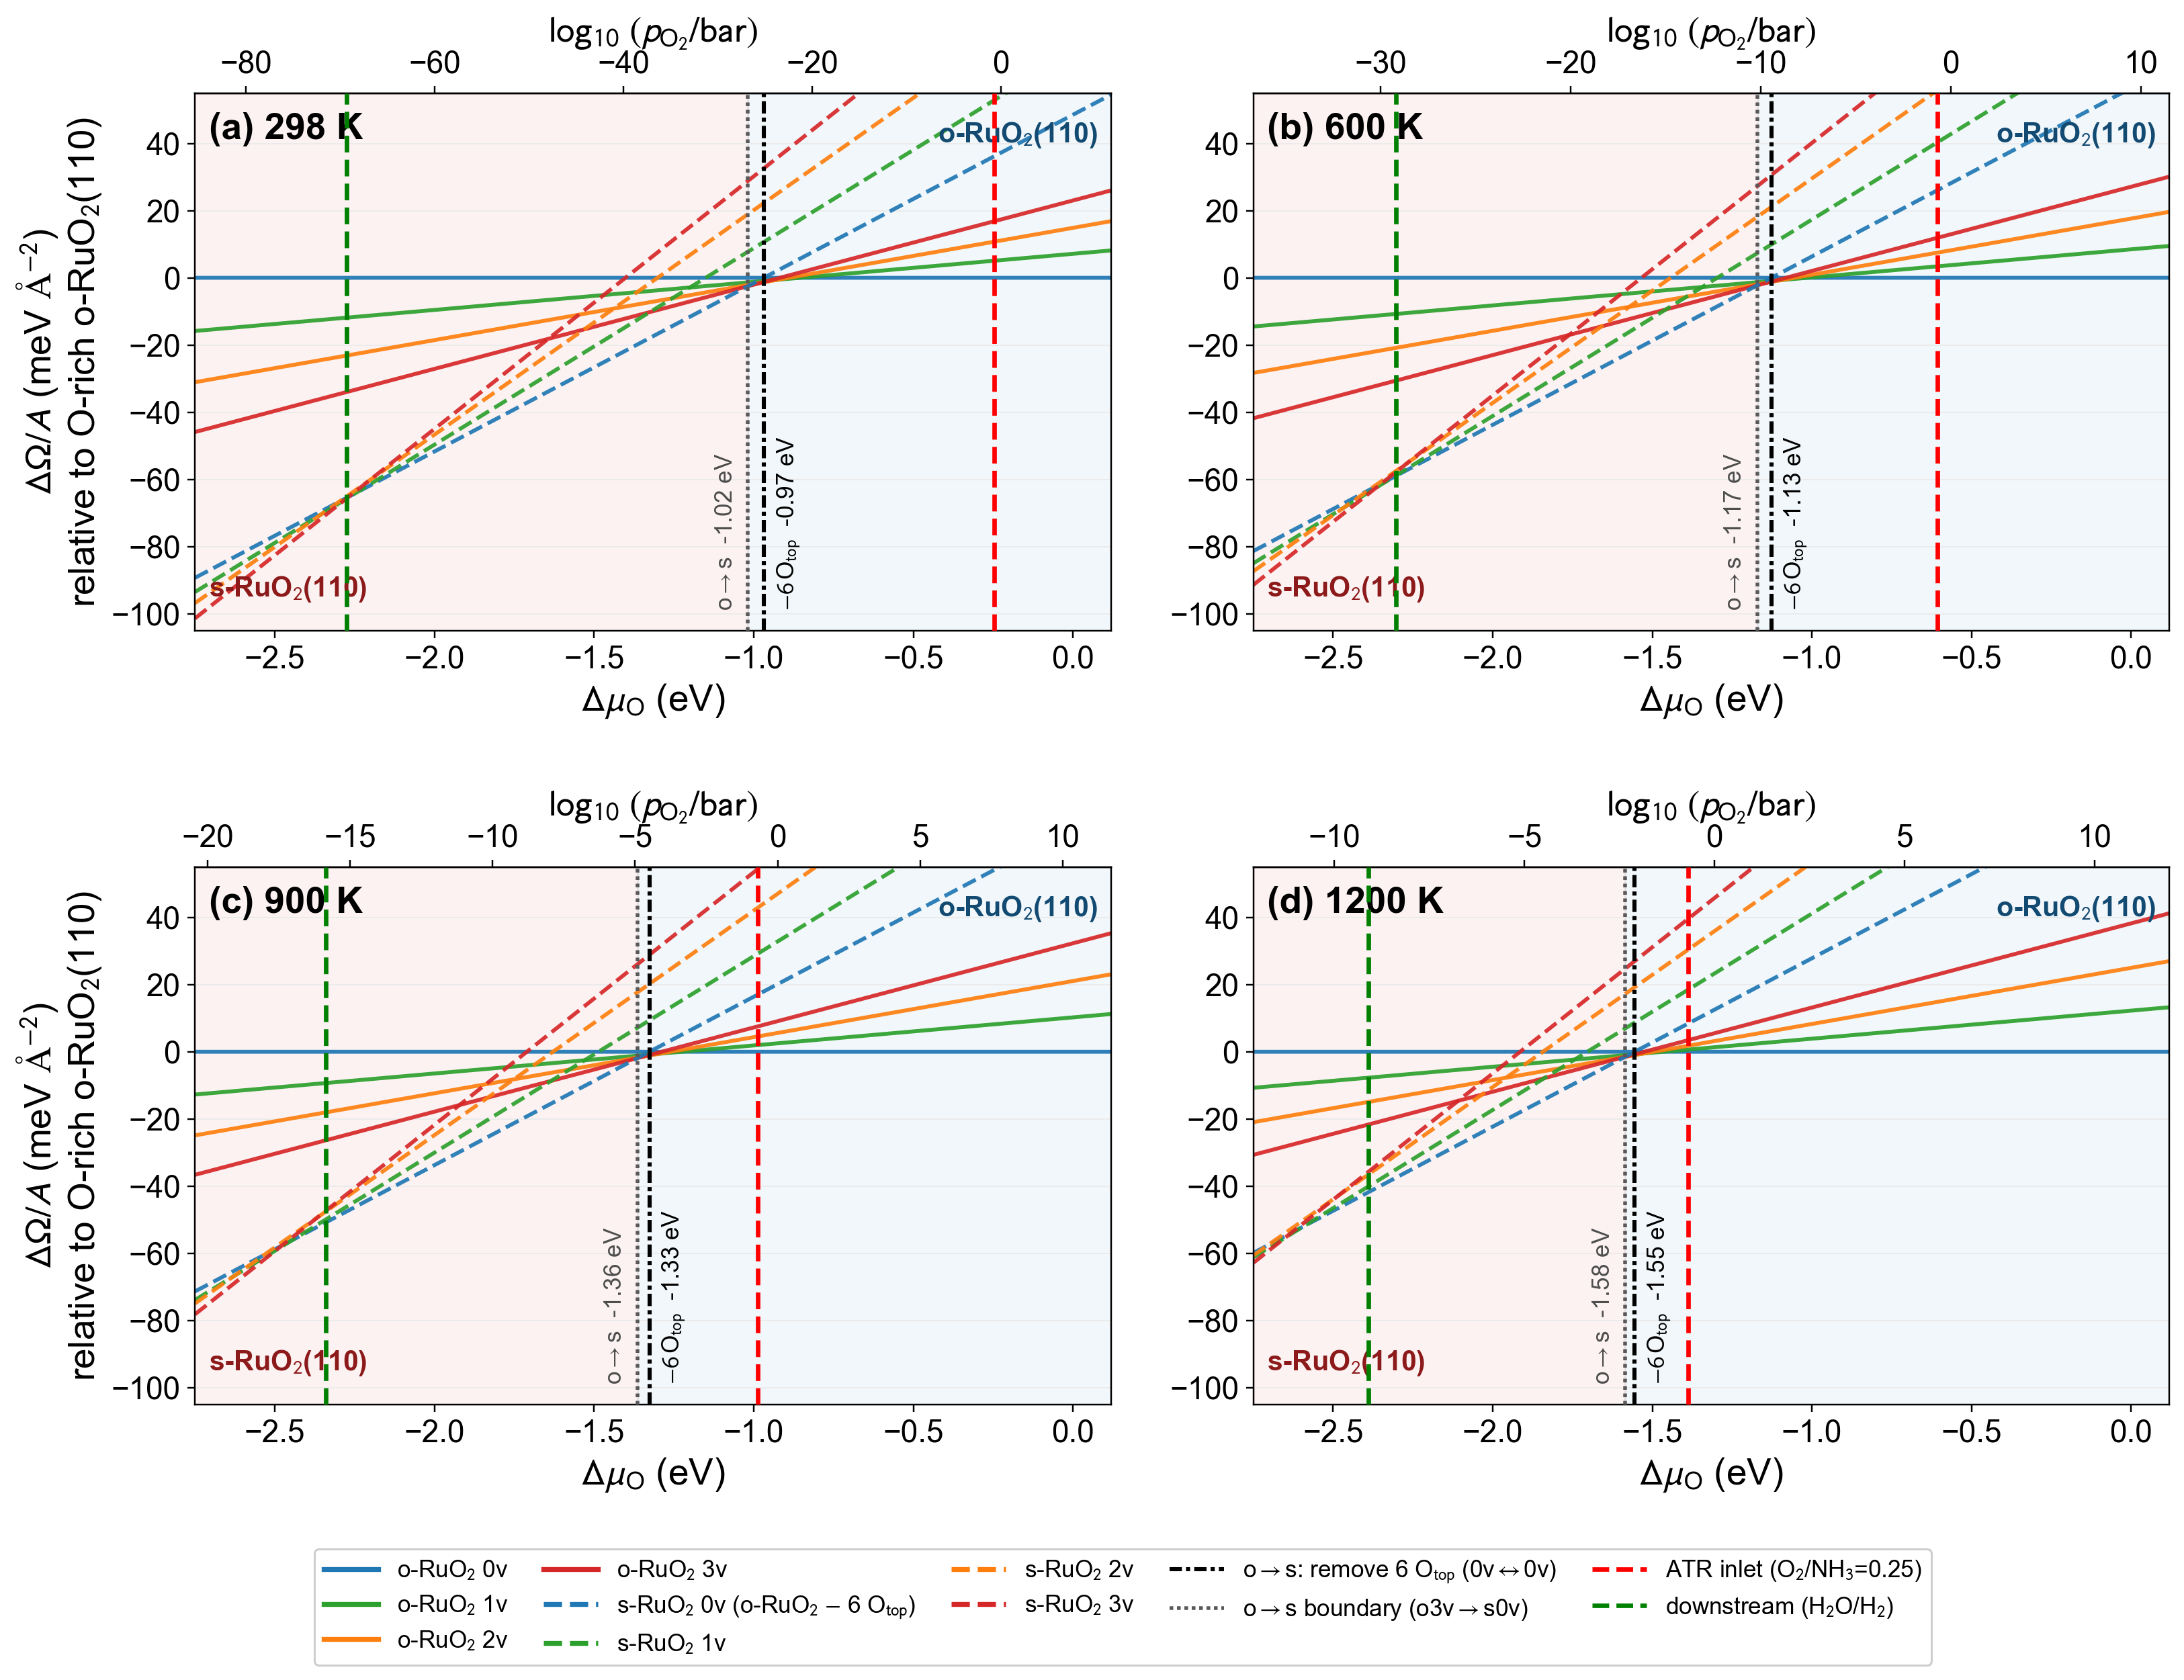
\includegraphics[width=\linewidth]{fig9_unified_states_2x2_dft.png}
  \caption{Relative surface grand potential $\Delta\Omega_k/A$ of the
  \textit{o}- and \textit{s}-RuO$_2$(110) terminations, all referenced to a single
  \textit{o}-RuO$_2$(110) 0v surface, at (a)~298, (b)~600, (c)~900 and (d)~1200~K.
  Solid lines, \textit{o}-RuO$_2$(110) $k$-vacancy surfaces (0--3v); dashed lines,
  \textit{s}-RuO$_2$(110) surfaces, with \textit{s}-RuO$_2$(110) 0v being
  \textit{o}-RuO$_2$(110) with its six on-top oxygens removed
  (Ru$_{36}$O$_{78}\rightarrow$Ru$_{36}$O$_{72}$). The black dash-dotted line marks
  the direct \textit{o}$\rightarrow$\textit{s} transition by removal of the six
  on-top oxygens (0v$\leftrightarrow$0v); the grey dotted line marks the
  \textit{o}$\rightarrow$\textit{s} transition between the most stable terminations
  (\textit{o}-RuO$_2$ 3v $\rightarrow$ \textit{s}-RuO$_2$ 0v). Red and green dashed verticals locate the
  ATR inlet ($\mathrm{O_2/NH_3}=0.25$) and downstream reforming
  ($\mathrm{H_2O/H_2}=10$) oxygen chemical potentials
  (Eqs.~\eqref{eq:inlet}--\eqref{eq:down}). Shaded bands indicate the
  \textit{s}-stable (left) and \textit{o}-stable (right) regions. The upper axis of
  each panel gives the corresponding oxygen partial pressure,
  $\log_{10}\!\left(p_{\mathrm{O_2}}/\mathrm{bar}\right)$ (Eq.~\eqref{eq:pO2}); all
  panels share a common axis.}
  \label{fig:unified}
\end{figure*}

\begin{figure*}[htbp]
  \centering
  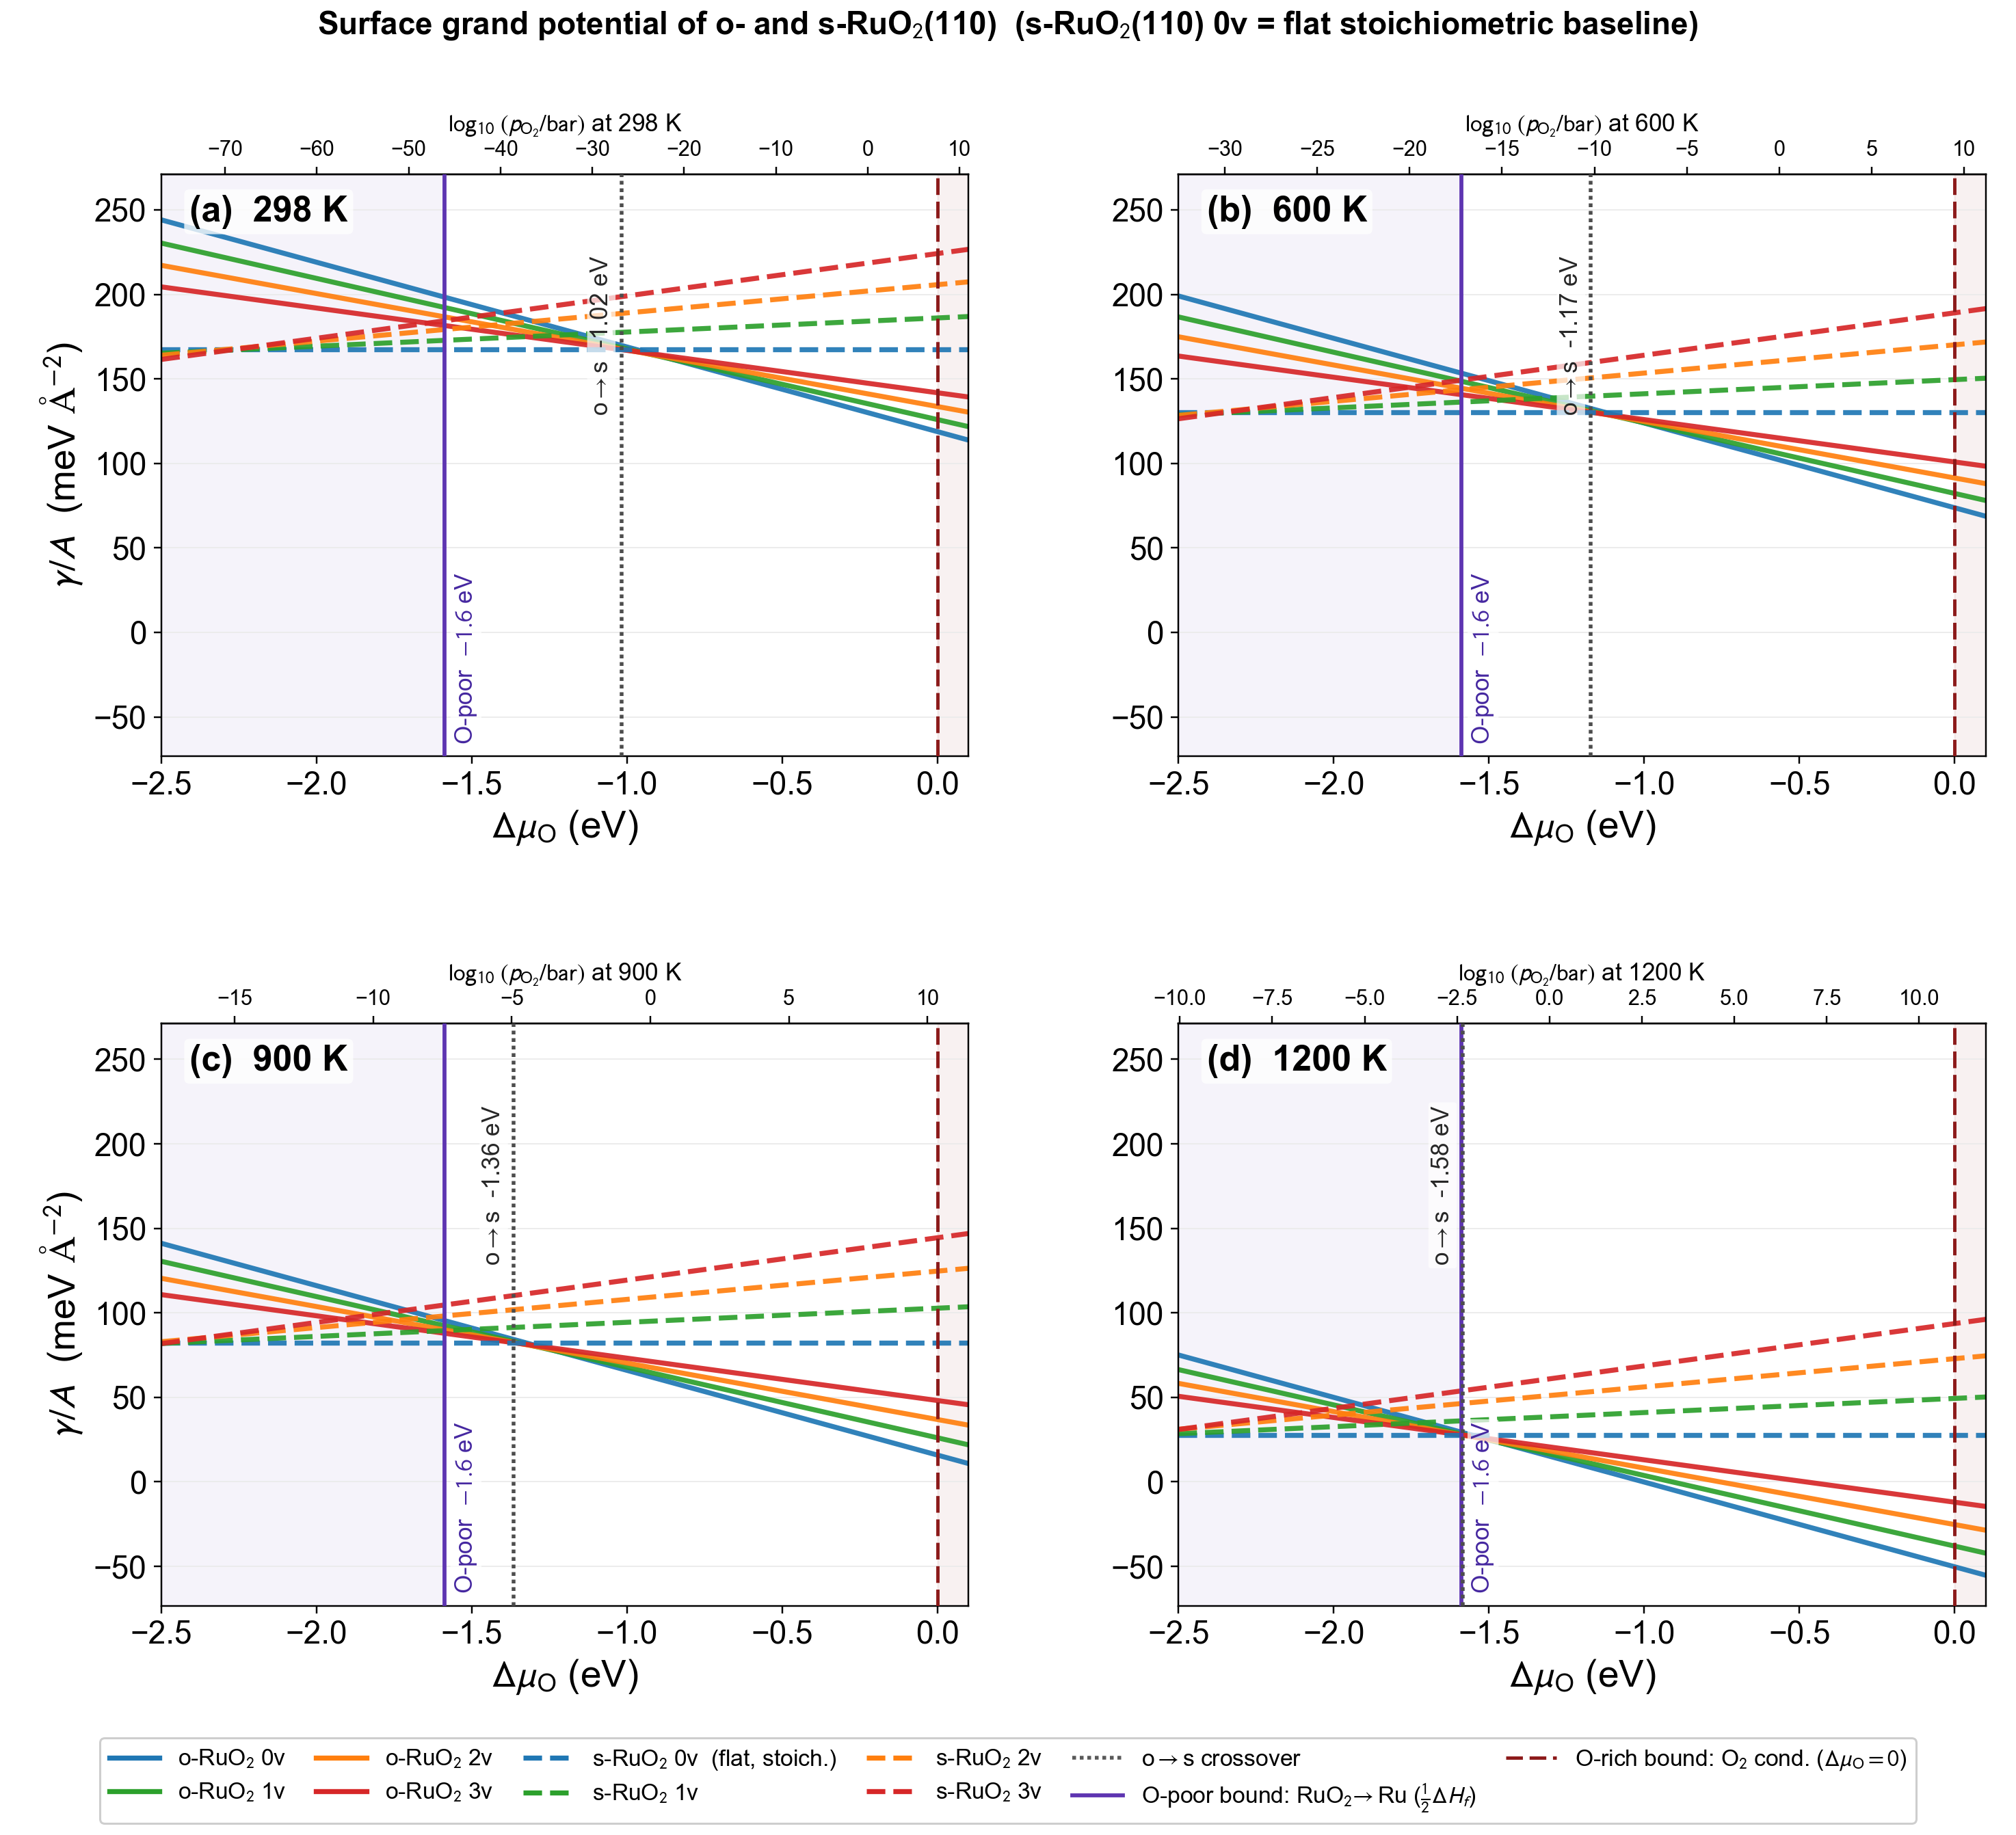
\includegraphics[width=\linewidth]{fig_bulk_referenced_2x2_dft.png}
  \caption{Surface grand potential of the \textit{o}- and
  \textit{s}-RuO$_2$(110) terminations referenced to bulk RuO$_2$ (absolute
  surface free energy $\gamma$) at (a)~298, (b)~600, (c)~900 and (d)~1200~K.
  Solid lines, \textit{o}-RuO$_2$(110) $k$-vacancy surfaces; dashed lines,
  \textit{s}-RuO$_2$(110); the stoichiometric \textit{s}-RuO$_2$(110) 0v surface
  is flat. The dotted line marks the \textit{o}$\rightarrow$\textit{s} boundary
  separating stable \textit{s}-RuO$_2$(110) (left) from \textit{o}-RuO$_2$(110)
  (right), identical to that of Figure~\ref{fig:unified}. Shaded bands are
  thermodynamically
  inaccessible: the oxygen-rich limit at $\Delta\mu_{\mathrm O}=0$ (O$_2$
  condensation) and the oxygen-poor limit at
  $\Delta\mu_{\mathrm O}=\tfrac{1}{2}\Delta H_f^{\,\mathrm{RuO_2}}\approx-1.60$~eV
  (decomposition to metallic Ru, Eq.~\eqref{eq:opoor}). The upper axis of each
  panel gives the corresponding oxygen partial pressure,
  $\log_{10}\!\left(p_{\mathrm{O_2}}/\mathrm{bar}\right)$, at that temperature
  (Eq.~\eqref{eq:pO2}). All panels share a common $\gamma$ axis.}
  \label{fig:bulkref}
\end{figure*}
  where this section
%  should appear (e.g. in the Supporting Information). Requires amsmath +
%  amssymb, which are already loaded in ATR NH3.tex.
%
%  FIGURE: the bulk-referenced grand-potential figure uses graphicx (already
%  loaded in ATR NH3.tex) and the image file fig_bulk_referenced_2x2_dft.png,
%  which is committed alongside this .tex at the project root.
%
%  OPTIONAL SI equation numbering (S11, S12, ...): add these two lines to
%  your PREAMBLE, before \begin{document}:
%     \renewcommand{\theequation}{S\arabic{equation}}
%     \setcounter{equation}{10}
%
%  NOTE (revtex twocolumn): the three wide displays (Svib, dOmega/A, log10)
%  can overflow a single column; wrap them in \begin{widetext}...\end{widetext}
%  or compile the SI in onecolumn if they run over.
% =====================================================================

\section*{Computational Details}

\subsection*{Electronic-structure calculations}
Spin-polarized density functional theory (DFT) calculations were performed with
the Perdew--Burke--Ernzerhof (PBE) exchange--correlation functional in the Vienna
\textit{Ab initio} Simulation Package (VASP), using the projector augmented-wave
method and a 430~eV plane-wave cutoff, as detailed in Section~2 of the main text.
The RuO$_2$(110) surfaces were modeled as $(2\times2)$ three-trilayer slabs and
the Ru(0001) surface as a $(4\times4)$ slab, each separated from its periodic
images by a vacuum gap.

\subsection*{Free-energy corrections}
The Gibbs free energy of every slab configuration used in the thermodynamic
analysis is evaluated from its DFT total energy $E_{\mathrm{DFT}}$ together with
the zero-point energy and vibrational (entropic) corrections obtained from the
harmonic vibrational frequencies $\nu_i$:
\begin{equation}
  G_{\mathrm{slab}}(T) = E_{\mathrm{DFT}} + E_{\mathrm{ZPE}}
  - T\,S_{\mathrm{vib}}(T)
  \label{eq:Gslab}
\end{equation}
\begin{equation}
  E_{\mathrm{ZPE}} = \tfrac{1}{2}\sum_i h\nu_i
  \label{eq:ZPE}
\end{equation}
\begin{equation}
  S_{\mathrm{vib}}(T) = k_{\mathrm B}\sum_i\left[
    \frac{h\nu_i/k_{\mathrm B}T}{e^{\,h\nu_i/k_{\mathrm B}T}-1}
    - \ln\!\left(1-e^{-h\nu_i/k_{\mathrm B}T}\right)\right]
  \label{eq:Svib}
\end{equation}
where $k_{\mathrm B}$ and $h$ are the Boltzmann and Planck constants. Because the
zero-point and vibrational-entropy terms are folded directly into
$G_{\mathrm{slab}}(T)$, the tabulated slab free energies are temperature
dependent (e.g., \textit{o}-RuO$_2$(110) 0v: $-817.70$~eV at $0$~K
$\rightarrow -837.48$~eV at $1200$~K), and no additional entropy term is applied
in the grand-potential expressions below. Vibrational frequencies of gas-phase
species were taken from the NIST Computational Chemistry Comparison and Benchmark
Database.

\subsection*{Oxygen reservoir chemical potential}
The surface exchanges lattice oxygen with a gas-phase O$_2$ reservoir. At
temperature $T$ and pressure $p$ the reservoir chemical potential varies with
pressure as
\begin{equation}
  \mu_{\mathrm{O_2}}(T,p) = \mu_{\mathrm{O_2}}(T,p^{0})
  + k_{\mathrm B}T\ln\!\left(p/p^{0}\right)
  \label{eq:muO2}
\end{equation}
and the oxygen chemical potential is one-half of it, referenced to the $0$~K DFT
O$_2$ energy:
\begin{equation}
  \mu_{\mathrm O}(T,p) = \tfrac{1}{2}\mu_{\mathrm{O_2}}(T,p)
  = \tfrac{1}{2}G_{\mathrm{O_2}}(0\,\mathrm{K}) + \Delta\mu_{\mathrm O}
  \label{eq:muO}
\end{equation}
\begin{equation}
  \Delta\mu_{\mathrm O} =
  \tfrac{1}{2}\left[G_{\mathrm{O_2}}(T) - G_{\mathrm{O_2}}(0\,\mathrm{K})\right]
  + \tfrac{1}{2}k_{\mathrm B}T\ln\!\left(p_{\mathrm{O_2}}/p^{0}\right)
  \label{eq:dmuO}
\end{equation}
so that $\Delta\mu_{\mathrm O}=0$ corresponds to gas-phase O$_2$ at $0$~K and more
negative $\Delta\mu_{\mathrm O}$ denotes more reducing conditions. The thermal term
$\tfrac{1}{2}[G_{\mathrm{O_2}}(T)-G_{\mathrm{O_2}}(0\,\mathrm{K})]$ is evaluated
directly from our calculated ideal-gas Gibbs free energy of O$_2$ (translational,
rotational, and vibrational contributions), giving $-0.23$, $-0.57$, $-0.93$, and
$-1.31$~eV per O atom at $298$, $600$, $900$, and $1200$~K, respectively.

\subsection*{Surface grand potential}
The grand potential of a slab open to the oxygen reservoir is
\begin{equation}
  \Omega = U - T\,S(T) - \sum_i \mu_i N_i
  \label{eq:Omega_gen}
\end{equation}
Using the slab free energy of Eq.~\eqref{eq:Gslab} for the $U-TS$ term and noting
that only oxygen is exchanged with the reservoir while ruthenium is conserved,
this becomes
\begin{equation}
  \Omega = G_{\mathrm{slab}}(T) - \mu_{\mathrm O} N_{\mathrm O}
  - \mu_{\mathrm{Ru}} N_{\mathrm{Ru}}
  \label{eq:Omega_surf}
\end{equation}
where $N_{\mathrm O}$ and $N_{\mathrm{Ru}}$ are the numbers of O and Ru atoms in
the cell. Because every termination contains the same $N_{\mathrm{Ru}}=36$, the
$\mu_{\mathrm{Ru}}N_{\mathrm{Ru}}$ term is identical across surfaces and cancels
when grand potentials are compared.

\subsection*{Relative (referenced) grand potential}
Terminations are compared through the grand potential of each $k$-vacancy surface
relative to a vacancy-free reference, per unit surface area $A$
($=119.70~\text{\AA}^{2}$ for the $(2\times2)$ cell):
\begin{equation}
  \frac{\Delta\Omega_k}{A} =
  \frac{\left[G_{\mathrm{slab}}^{(k)}(T)
  - G_{\mathrm{slab}}^{(\mathrm{ref})}(T)\right]
  + n_{\mathrm{vac}}\left(\tfrac{1}{2}G_{\mathrm{O_2}}(0\,\mathrm{K})
  + \Delta\mu_{\mathrm O}\right)}{A}
  \label{eq:dOmega}
\end{equation}
where $n_{\mathrm{vac}} = N_{\mathrm O}^{(\mathrm{ref})} - N_{\mathrm O}^{(k)}$ is
the number of oxygen atoms removed relative to the reference, so the slope of each
line, $n_{\mathrm{vac}}/A$, is the areal density of released oxygen. The
referencing subtracts a common term ($\mu_{\mathrm{Ru}}N_{\mathrm{Ru}}$ and the
bulk contribution), making $\Delta\Omega$ independent of the ruthenium reference.
This relative construction is thermodynamically equivalent to the absolute surface
free energy $\gamma = (1/A)[\,G_{\mathrm{slab}} - N_{\mathrm{Ru}}\,g^{\mathrm{bulk}}_{\mathrm{RuO_2}}
- (N_{\mathrm O}-2N_{\mathrm{Ru}})\,\mu_{\mathrm O}\,]$ of Reuter and Scheffler
[K.~Reuter and M.~Scheffler, Phys.\ Rev.\ B \textbf{65}, 035406 (2001)]: because
every termination shares the same $N_{\mathrm{Ru}}$, referencing to the
\textit{o}-RuO$_2$(110) 0v surface removes the $\mu_{\mathrm{Ru}}$ term by
construction, instead of through the bulk-equilibrium constraint
$\mu_{\mathrm{Ru}}+2\mu_{\mathrm O}=g^{\mathrm{bulk}}_{\mathrm{RuO_2}}$ that references
$\gamma$ to bulk RuO$_2$; both choices leave every crossover and vacancy-formation
threshold unchanged.
This unified construction is shown in Figure~\ref{fig:unified}, in which all
terminations share the single \textit{o}-RuO$_2$(110) 0v reference, using the fact
that \textit{s}-RuO$_2$(110) 0v is \textit{o}-RuO$_2$(110) with its six on-top
oxygens removed (Ru$_{36}$O$_{78} \rightarrow$ Ru$_{36}$O$_{72}$,
$n_{\mathrm{vac}}=6$). The equivalent diagram referenced to bulk RuO$_2$ is shown
in Figure~\ref{fig:bulkref}; presenting the two reference choices side by side
demonstrates that the \textit{o}$\rightarrow$\textit{s} crossover and
vacancy-formation thresholds are independent of the reference.

\subsection*{Operating oxygen chemical potentials}
The ATR inlet is set by a fixed feed oxygen partial pressure
(O$_2$/NH$_3 = 0.25 \rightarrow p_{\mathrm{O_2}} = 0.2$~bar):
\begin{equation}
  \Delta\mu_{\mathrm O}^{\,\mathrm{inlet}} =
  \tfrac{1}{2}\left[G_{\mathrm{O_2}}(T) - G_{\mathrm{O_2}}(0\,\mathrm{K})\right]
  + \tfrac{1}{2}k_{\mathrm B}T\ln\!\left(p_{\mathrm{O_2}}/p^{0}\right)
  \label{eq:inlet}
\end{equation}
The downstream reforming potential is fixed by the
H$_2 + \tfrac{1}{2}$O$_2 \rightleftharpoons$ H$_2$O equilibrium, and is
independent of the O$_2$ reference:
\begin{equation}
  \Delta\mu_{\mathrm O}^{\,\mathrm{down}} =
  \left[G_{\mathrm{H_2O}}(T) - G_{\mathrm{H_2}}(T)\right]
  - \tfrac{1}{2}G_{\mathrm{O_2}}(0\,\mathrm{K})
  + k_{\mathrm B}T\ln\!\left(p_{\mathrm{H_2O}}/p_{\mathrm{H_2}}\right)
  \label{eq:down}
\end{equation}
evaluated at $p_{\mathrm{H_2O}}/p_{\mathrm{H_2}}=10$. The upper axes of
Figures~\ref{fig:unified} and~\ref{fig:bulkref} convert $\Delta\mu_{\mathrm O}$
into an equivalent O$_2$ partial pressure by
inverting Eq.~\eqref{eq:dmuO}:
\begin{equation}
  \log_{10}\!\left(p_{\mathrm{O_2}}/p^{0}\right) =
  \frac{\Delta\mu_{\mathrm O}
  - \tfrac{1}{2}\left(G_{\mathrm{O_2}}(T) - G_{\mathrm{O_2}}(0\,\mathrm{K})\right)}
       {\tfrac{1}{2}k_{\mathrm B}T\ln 10}
  \label{eq:pO2}
\end{equation}
with $p^{0}=1$~bar the standard-state pressure.

\subsection*{Bulk-referenced surface stability and correlation to ATR conditions}
Referencing the surface grand potential to bulk RuO$_2$ rather than to the
\textit{o}-RuO$_2$(110) 0v surface converts the relative curves of
Eq.~\eqref{eq:dOmega} into absolute surface free energies
$\gamma(\Delta\mu_{\mathrm O})$ and, in addition, places the accessible oxygen
chemical potential on a physical scale bounded by two limits. The oxygen-rich
limit is fixed by O$_2$ condensation, $\Delta\mu_{\mathrm O}=0$; the oxygen-poor
limit is fixed by decomposition of the oxide into metallic ruthenium,
$\mathrm{RuO_2}\rightarrow\mathrm{Ru}+\mathrm{O_2}$, which occurs when
\begin{equation}
  \Delta\mu_{\mathrm O}^{\,\mathrm{poor}} =
  \tfrac{1}{2}\,\Delta H_f^{\,\mathrm{RuO_2}} \approx -1.60~\mathrm{eV},
  \label{eq:opoor}
\end{equation}
using the experimental heat of formation $\Delta H_f^{\,\mathrm{RuO_2}}=-3.19$~eV
[NIST--JANAF; consistent with the value adopted by Reuter and Scheffler,
Phys.\ Rev.\ B \textbf{68}, 045407 (2003)]. Because $\Delta\mu_{\mathrm O}$
already carries the full temperature and pressure dependence of the O$_2$
reservoir (Eq.~\eqref{eq:dmuO}), this decomposition bound is temperature
independent. Figure~\ref{fig:bulkref} shows the resulting diagram at 298, 600,
900 and 1200~K. In this reference the stoichiometric \textit{s}-RuO$_2$(110) 0v
surface ($N_{\mathrm O}=2N_{\mathrm{Ru}}$) is flat, whereas every oxygen-rich
termination slopes downward with a slope equal to its excess-oxygen areal
density, $-(N_{\mathrm O}-2N_{\mathrm{Ru}})/A$
($-50.1$~meV\,\AA$^{-2}$\,eV$^{-1}$ for the six on-top oxygens of
\textit{o}-RuO$_2$(110) 0v). Every \textit{o}$\rightarrow$\textit{s} crossover is
numerically identical to that of the \textit{o}-RuO$_2$(110)-referenced diagram
(Figure~\ref{fig:unified}), confirming that the surface phase
boundaries are independent of the chosen reference.

At any oxygen potential the thermodynamically stable surface is simply the
termination of lowest $\gamma$. On the oxygen-rich (right) side of each panel this
is the steeply sloped, oxygen-covered \textit{o}-RuO$_2$(110) surface; on the
oxygen-poor (left) side it is the flat stoichiometric \textit{s}-RuO$_2$(110)
0v surface. The dotted vertical line marks the oxygen potential at which the two are
equally stable---the \textit{o}$\rightarrow$\textit{s} boundary---at
$\Delta\mu_{\mathrm O}=-1.02$, $-1.17$, $-1.36$ and $-1.58$~eV for 298, 600, 900
and 1200~K, respectively. To the right of this line the oxidised
\textit{o}-RuO$_2$(110) surface is stable; to the left, the surface has released its
on-top oxygens to become the reduced \textit{s}-RuO$_2$(110) termination. The closer
an operating point sits to this boundary, the smaller the free-energy margin (a few
meV\,\AA$^{-2}$) between the two terminations, so near it the oxidised and reduced
surfaces are effectively degenerate within DFT accuracy.

Superimposing the ATR operating potentials of
Eqs.~\eqref{eq:inlet}--\eqref{eq:down} on this stability window links the surface
oxidation state directly to reactor position. At the ATR inlet
($\mathrm{O_2/NH_3}=0.25$, $p_{\mathrm{O_2}}=0.2$~bar) the oxygen potential
$\Delta\mu_{\mathrm O}^{\,\mathrm{inlet}}$ ranges from $-0.25$~eV at 298~K to
$-1.39$~eV at 1200~K; it lies inside the RuO$_2$ stability window at every
temperature and on the oxygen-rich side of the
\textit{o}$\rightarrow$\textit{s} crossover, so the inlet surface is the
oxygen-covered \textit{o}-RuO$_2$(110) termination. Downstream, once the
$\mathrm{H_2O/H_2}$ reforming equilibrium is established
($\Delta\mu_{\mathrm O}^{\,\mathrm{down}}\approx-2.3$~eV at
$p_{\mathrm{H_2O}}/p_{\mathrm{H_2}}=10$), the potential falls \emph{below} the
oxide-decomposition bound of Eq.~\eqref{eq:opoor} at all temperatures: the
reducing reforming atmosphere drives the termination through the
\textit{s}-RuO$_2$(110) surface and ultimately toward metallic ruthenium. The
\textit{o}$\rightarrow$\textit{s} crossover ($-1.02$ to $-1.58$~eV) sits between
these two operating points, so a catalyst particle necessarily evolves from the
selective, oxygen-rich \textit{o}-RuO$_2$ surface near the inlet to the reduced
\textit{s}-RuO$_2$ surface as ammonia is consumed and the local gas becomes
reducing. Increasing temperature compresses this window: at 1200~K the inlet
potential ($-1.39$~eV), the \textit{o}$\rightarrow$\textit{s} crossover
($-1.58$~eV) and the decomposition bound ($-1.60$~eV) nearly coincide, so the
reduced surface---and eventually metallic Ru---becomes accessible even close to
the inlet, consistent with the loss of N$_2$ selectivity observed at high
temperature.

Reading these transitions on the equivalent oxygen-pressure scale (upper axes of
Figure~\ref{fig:bulkref}, Eq.~\eqref{eq:pO2}) makes the reactor gradient
explicit. Table~\ref{tab:po2markers} lists the oxygen partial pressure
$p_{\mathrm{O_2}}$ at the inlet, at the \textit{o}$\rightarrow$\textit{s}
crossover, at the oxide-decomposition bound and at the downstream reforming
point. As O$_2$ is consumed along the bed the local oxygen potential sweeps
monotonically toward lower $p_{\mathrm{O_2}}$, so a catalyst particle crosses
these markers in sequence: the oxygen-covered \textit{o}-RuO$_2$(110)
termination at the inlet, the \textit{o}$\rightarrow$\textit{s} transition once
$p_{\mathrm{O_2}}$ has dropped by the margin listed in the final column, and
finally reduction past the decomposition bound in the reforming zone. This
oxidative margin collapses from $\sim$26 orders of magnitude in
$p_{\mathrm{O_2}}$ at 298~K to only $\sim$1.7 at 1200~K, where the crossover and
the decomposition bound become numerically coincident
($p_{\mathrm{O_2}}\approx10^{-2.4}$~bar). The oxygen-covered, N$_2$-selective
surface therefore persists over essentially the entire bed at low temperature
but is confined to a thin zone near the inlet at high temperature, providing a
thermodynamic rationale for the loss of N$_2$ selectivity as temperature
increases.

\begin{table*}[htbp]
  \centering
  \caption{Equivalent oxygen partial pressure $p_{\mathrm{O_2}}$ (bar) at the
  ATR inlet, the \textit{o}$\rightarrow$\textit{s} crossover, the oxygen-poor
  (decomposition) bound and the downstream reforming point, obtained from the
  operating potentials (Eqs.~\eqref{eq:inlet}--\eqref{eq:down}) through
  Eq.~\eqref{eq:pO2}. The final column is the oxidative margin: the drop in
  $p_{\mathrm{O_2}}$ (orders of magnitude) between the inlet and the
  \textit{o}$\rightarrow$\textit{s} crossover.}
  \label{tab:po2markers}
  \begin{tabular}{cccccc}
    \hline
    $T$ (K) & inlet & \textit{o}$\rightarrow$\textit{s} &
    O-poor ($\rightarrow$Ru) & downstream &
    inlet$\rightarrow$\,\textit{o}$\rightarrow$\textit{s} \\
     & (bar) & (bar) & (bar) & (bar) & (decades) \\
    \hline
    298  & $0.2$ & $10^{-27}$  & $10^{-46}$  & $10^{-69}$  & 26  \\
    600  & $0.2$ & $10^{-10}$  & $10^{-17}$  & $10^{-29}$  & 9.5 \\
    900  & $0.2$ & $10^{-4.9}$ & $10^{-7.5}$ & $10^{-16}$  & 4.2 \\
    1200 & $0.2$ & $10^{-2.4}$ & $10^{-2.4}$ & $10^{-9.1}$ & 1.7 \\
    \hline
  \end{tabular}
\end{table*}

\begin{figure*}[htbp]
  \centering
  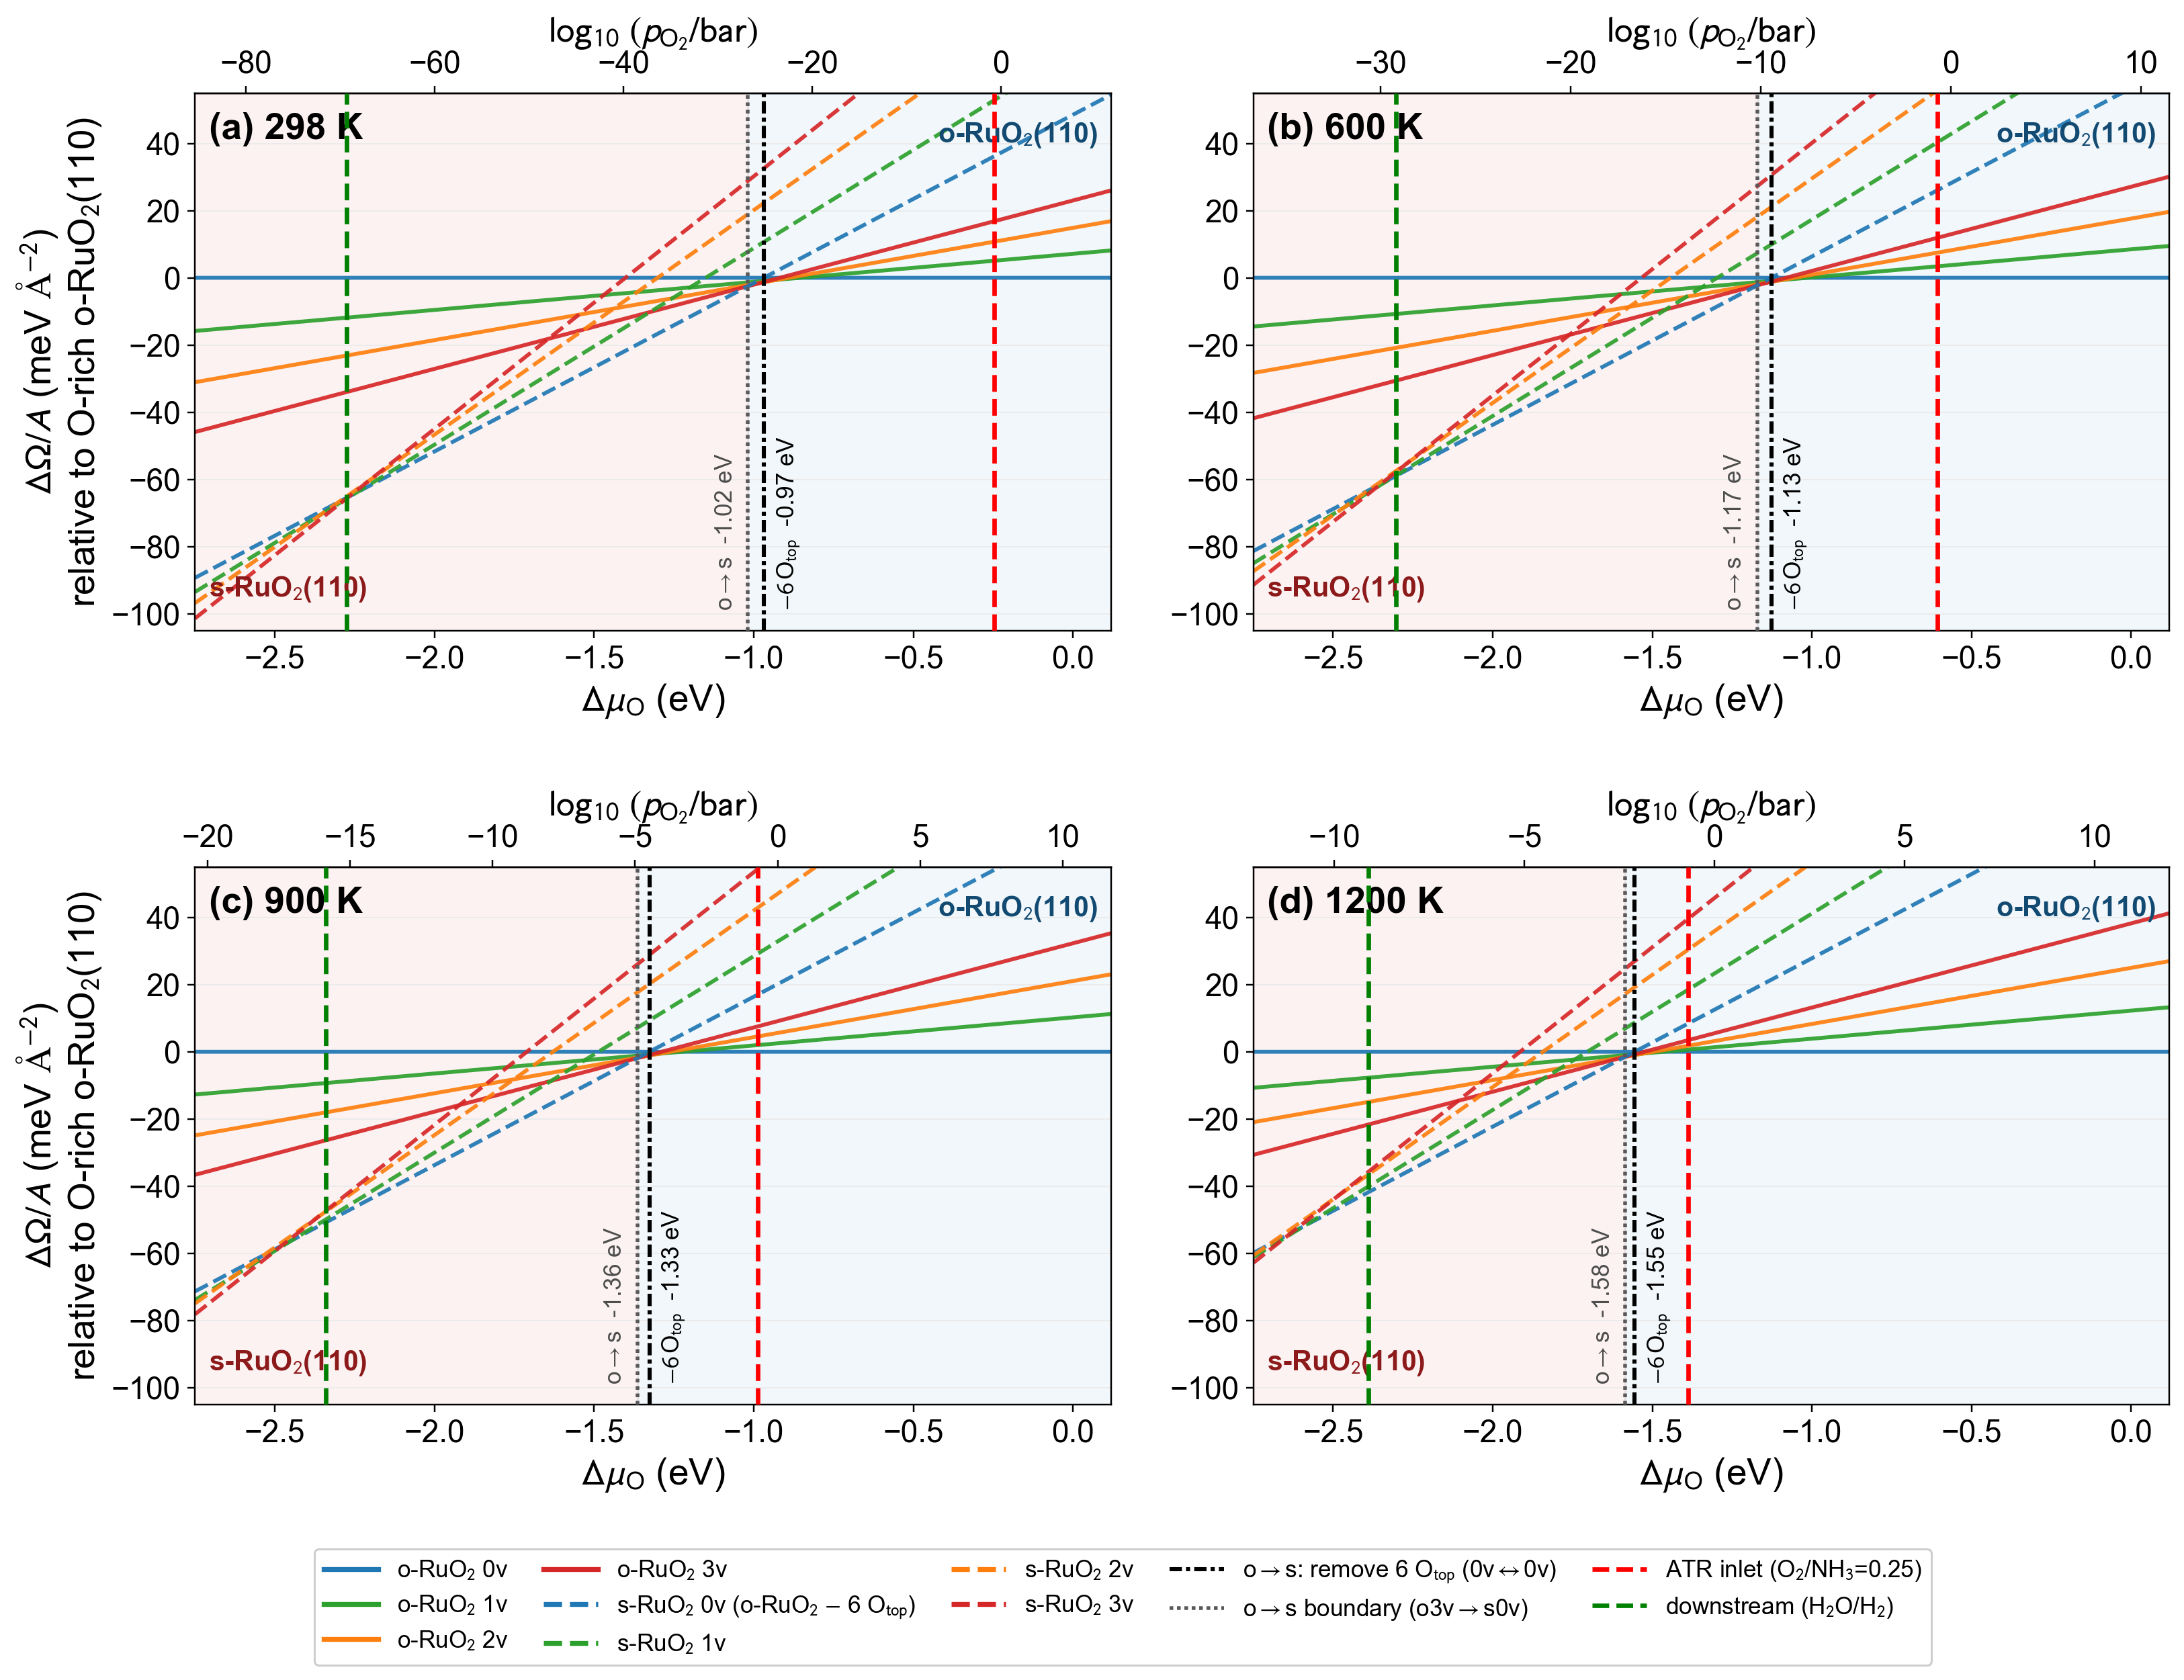
\includegraphics[width=\linewidth]{fig9_unified_states_2x2_dft.png}
  \caption{Relative surface grand potential $\Delta\Omega_k/A$ of the
  \textit{o}- and \textit{s}-RuO$_2$(110) terminations, all referenced to a single
  \textit{o}-RuO$_2$(110) 0v surface, at (a)~298, (b)~600, (c)~900 and (d)~1200~K.
  Solid lines, \textit{o}-RuO$_2$(110) $k$-vacancy surfaces (0--3v); dashed lines,
  \textit{s}-RuO$_2$(110) surfaces, with \textit{s}-RuO$_2$(110) 0v being
  \textit{o}-RuO$_2$(110) with its six on-top oxygens removed
  (Ru$_{36}$O$_{78}\rightarrow$Ru$_{36}$O$_{72}$). The black dash-dotted line marks
  the direct \textit{o}$\rightarrow$\textit{s} transition by removal of the six
  on-top oxygens (0v$\leftrightarrow$0v); the grey dotted line marks the
  \textit{o}$\rightarrow$\textit{s} transition between the most stable terminations
  (\textit{o}-RuO$_2$ 3v $\rightarrow$ \textit{s}-RuO$_2$ 0v). Red and green dashed verticals locate the
  ATR inlet ($\mathrm{O_2/NH_3}=0.25$) and downstream reforming
  ($\mathrm{H_2O/H_2}=10$) oxygen chemical potentials
  (Eqs.~\eqref{eq:inlet}--\eqref{eq:down}). Shaded bands indicate the
  \textit{s}-stable (left) and \textit{o}-stable (right) regions. The upper axis of
  each panel gives the corresponding oxygen partial pressure,
  $\log_{10}\!\left(p_{\mathrm{O_2}}/\mathrm{bar}\right)$ (Eq.~\eqref{eq:pO2}); all
  panels share a common axis.}
  \label{fig:unified}
\end{figure*}

\begin{figure*}[htbp]
  \centering
  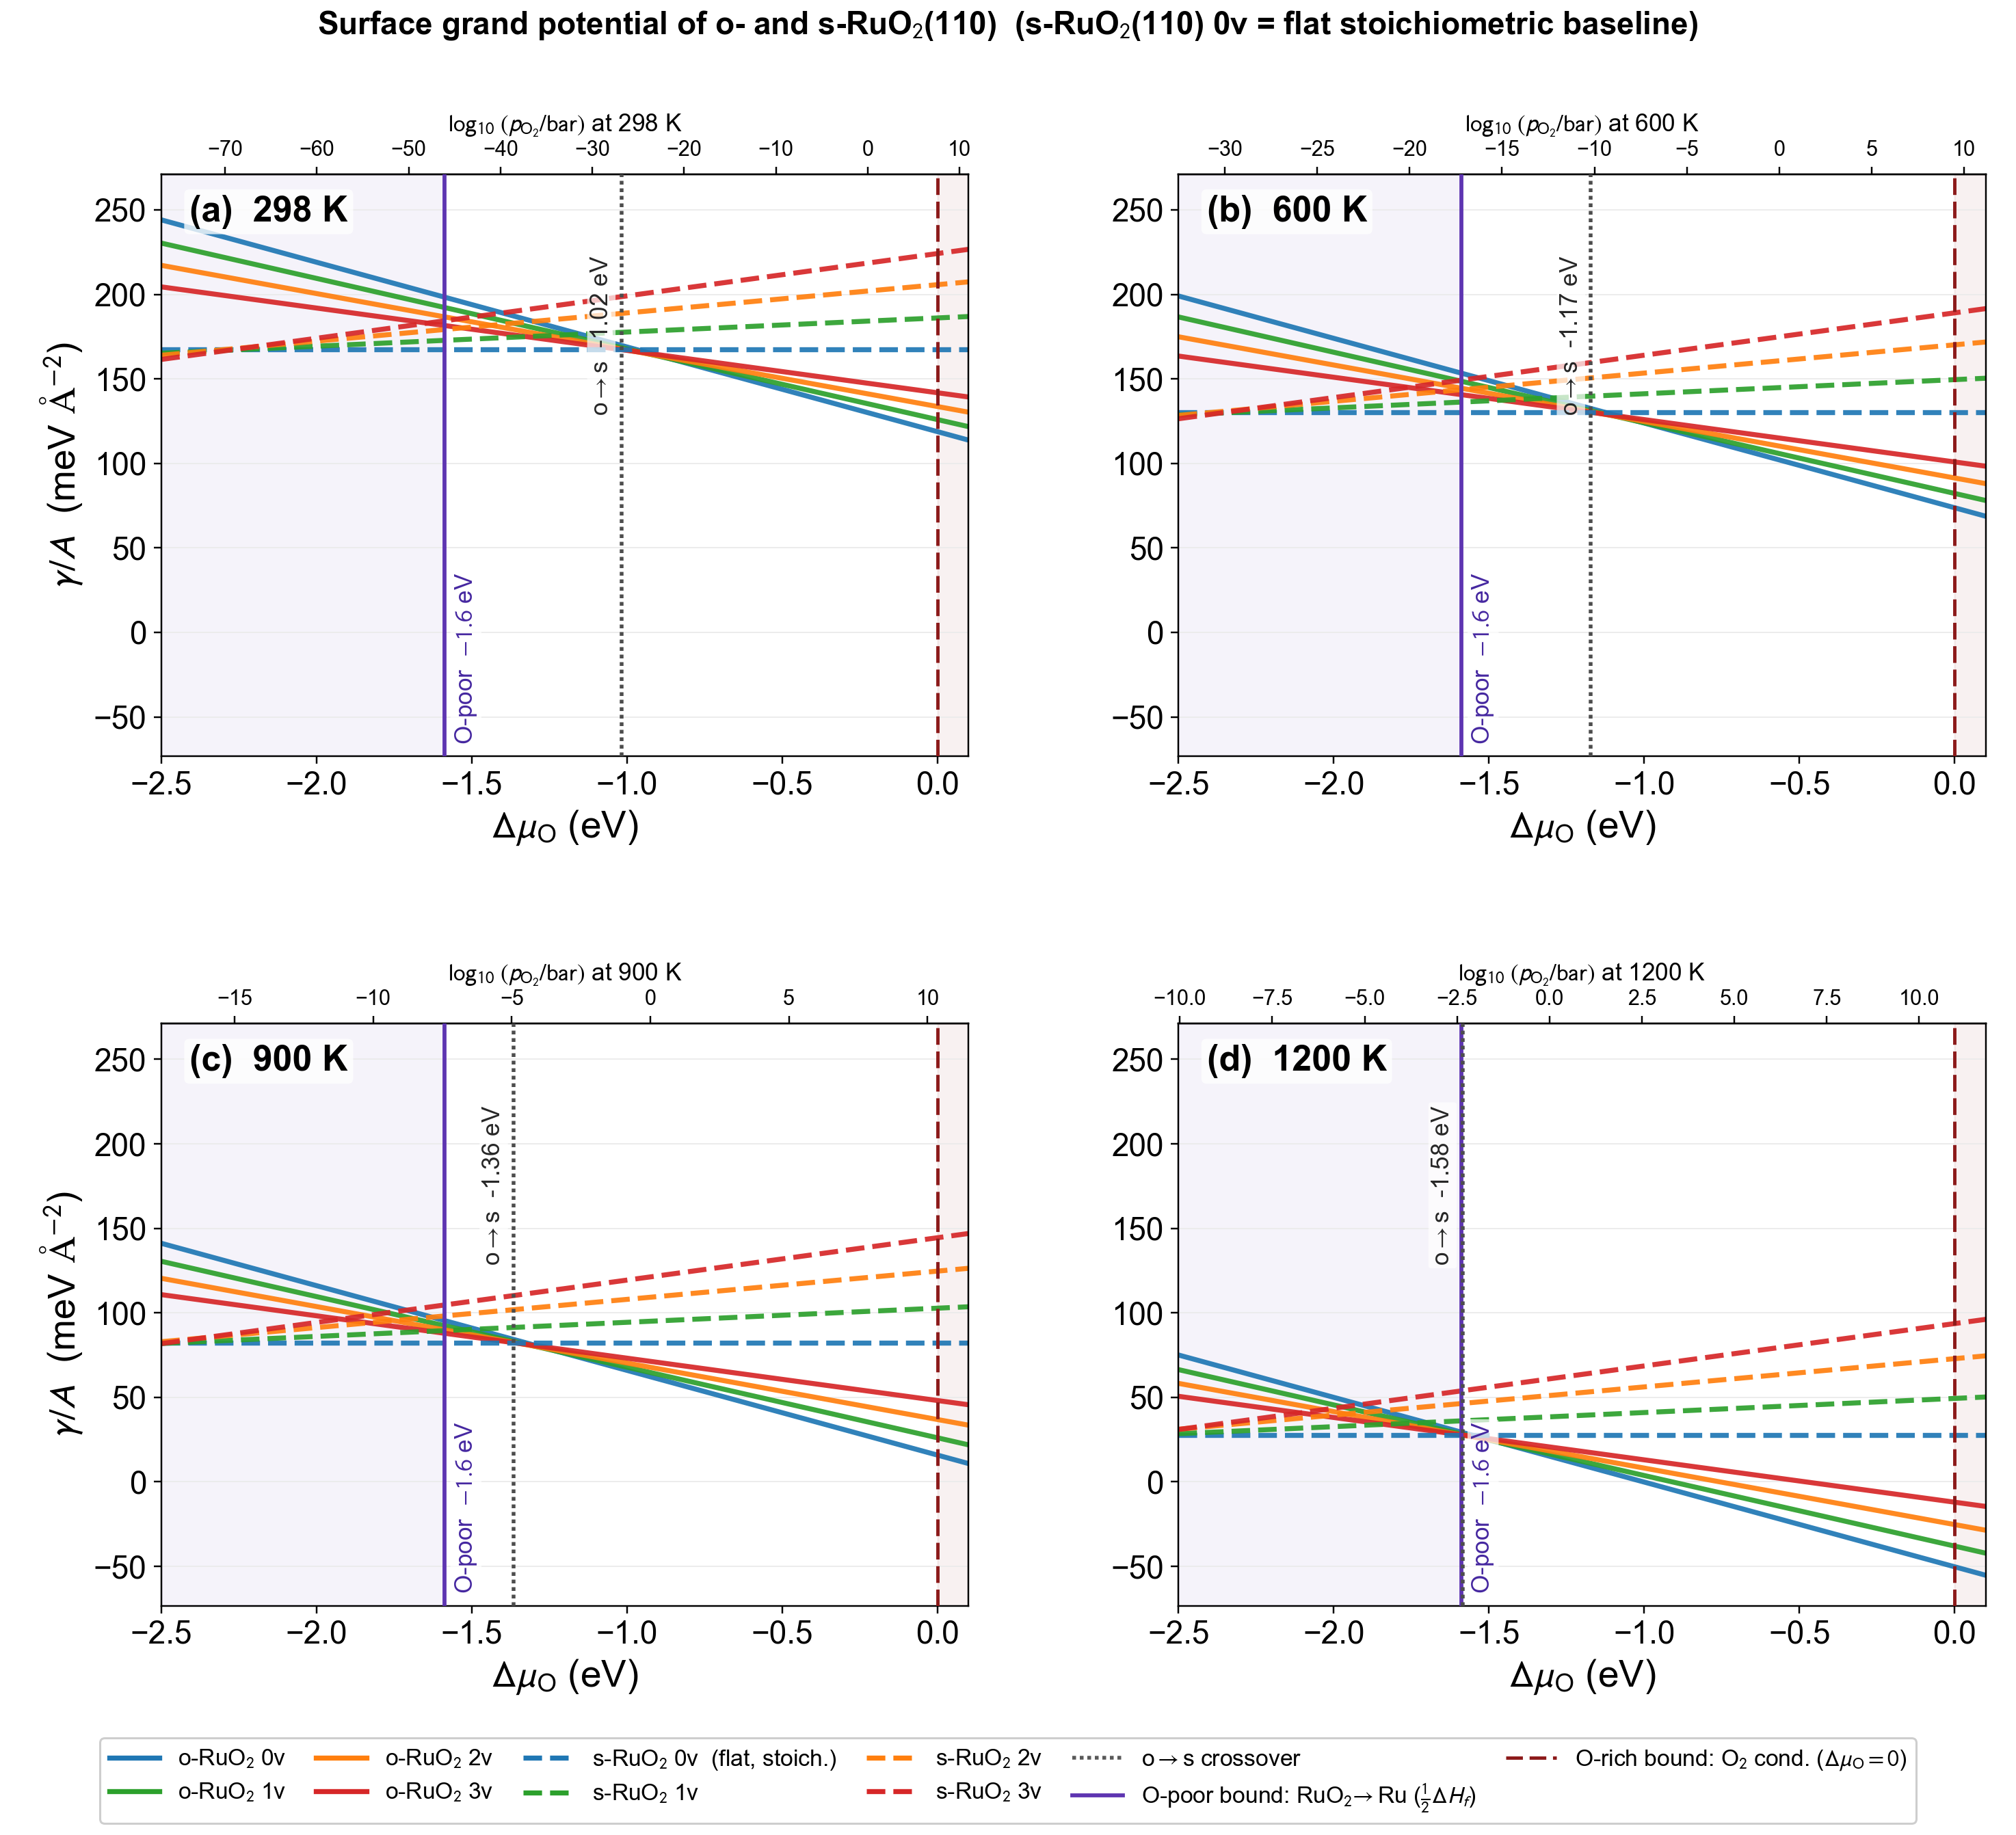
\includegraphics[width=\linewidth]{fig_bulk_referenced_2x2_dft.png}
  \caption{Surface grand potential of the \textit{o}- and
  \textit{s}-RuO$_2$(110) terminations referenced to bulk RuO$_2$ (absolute
  surface free energy $\gamma$) at (a)~298, (b)~600, (c)~900 and (d)~1200~K.
  Solid lines, \textit{o}-RuO$_2$(110) $k$-vacancy surfaces; dashed lines,
  \textit{s}-RuO$_2$(110); the stoichiometric \textit{s}-RuO$_2$(110) 0v surface
  is flat. The dotted line marks the \textit{o}$\rightarrow$\textit{s} boundary
  separating stable \textit{s}-RuO$_2$(110) (left) from \textit{o}-RuO$_2$(110)
  (right), identical to that of Figure~\ref{fig:unified}. Shaded bands are
  thermodynamically
  inaccessible: the oxygen-rich limit at $\Delta\mu_{\mathrm O}=0$ (O$_2$
  condensation) and the oxygen-poor limit at
  $\Delta\mu_{\mathrm O}=\tfrac{1}{2}\Delta H_f^{\,\mathrm{RuO_2}}\approx-1.60$~eV
  (decomposition to metallic Ru, Eq.~\eqref{eq:opoor}). The upper axis of each
  panel gives the corresponding oxygen partial pressure,
  $\log_{10}\!\left(p_{\mathrm{O_2}}/\mathrm{bar}\right)$, at that temperature
  (Eq.~\eqref{eq:pO2}). All panels share a common $\gamma$ axis.}
  \label{fig:bulkref}
\end{figure*}
  where this section
%  should appear (e.g. in the Supporting Information). Requires amsmath +
%  amssymb, which are already loaded in ATR NH3.tex.
%
%  FIGURE: the bulk-referenced grand-potential figure uses graphicx (already
%  loaded in ATR NH3.tex) and the image file fig_bulk_referenced_2x2_dft.png,
%  which is committed alongside this .tex at the project root.
%
%  OPTIONAL SI equation numbering (S11, S12, ...): add these two lines to
%  your PREAMBLE, before \begin{document}:
%     \renewcommand{\theequation}{S\arabic{equation}}
%     \setcounter{equation}{10}
%
%  NOTE (revtex twocolumn): the three wide displays (Svib, dOmega/A, log10)
%  can overflow a single column; wrap them in \begin{widetext}...\end{widetext}
%  or compile the SI in onecolumn if they run over.
% =====================================================================

\section*{Computational Details}

\subsection*{Electronic-structure calculations}
Spin-polarized density functional theory (DFT) calculations were performed with
the Perdew--Burke--Ernzerhof (PBE) exchange--correlation functional in the Vienna
\textit{Ab initio} Simulation Package (VASP), using the projector augmented-wave
method and a 430~eV plane-wave cutoff, as detailed in Section~2 of the main text.
The RuO$_2$(110) surfaces were modeled as $(2\times2)$ three-trilayer slabs and
the Ru(0001) surface as a $(4\times4)$ slab, each separated from its periodic
images by a vacuum gap.

\subsection*{Free-energy corrections}
The Gibbs free energy of every slab configuration used in the thermodynamic
analysis is evaluated from its DFT total energy $E_{\mathrm{DFT}}$ together with
the zero-point energy and vibrational (entropic) corrections obtained from the
harmonic vibrational frequencies $\nu_i$:
\begin{equation}
  G_{\mathrm{slab}}(T) = E_{\mathrm{DFT}} + E_{\mathrm{ZPE}}
  - T\,S_{\mathrm{vib}}(T)
  \label{eq:Gslab}
\end{equation}
\begin{equation}
  E_{\mathrm{ZPE}} = \tfrac{1}{2}\sum_i h\nu_i
  \label{eq:ZPE}
\end{equation}
\begin{equation}
  S_{\mathrm{vib}}(T) = k_{\mathrm B}\sum_i\left[
    \frac{h\nu_i/k_{\mathrm B}T}{e^{\,h\nu_i/k_{\mathrm B}T}-1}
    - \ln\!\left(1-e^{-h\nu_i/k_{\mathrm B}T}\right)\right]
  \label{eq:Svib}
\end{equation}
where $k_{\mathrm B}$ and $h$ are the Boltzmann and Planck constants. Because the
zero-point and vibrational-entropy terms are folded directly into
$G_{\mathrm{slab}}(T)$, the tabulated slab free energies are temperature
dependent (e.g., \textit{o}-RuO$_2$(110) 0v: $-817.70$~eV at $0$~K
$\rightarrow -837.48$~eV at $1200$~K), and no additional entropy term is applied
in the grand-potential expressions below. Vibrational frequencies of gas-phase
species were taken from the NIST Computational Chemistry Comparison and Benchmark
Database.

\subsection*{Oxygen reservoir chemical potential}
The surface exchanges lattice oxygen with a gas-phase O$_2$ reservoir. At
temperature $T$ and pressure $p$ the reservoir chemical potential varies with
pressure as
\begin{equation}
  \mu_{\mathrm{O_2}}(T,p) = \mu_{\mathrm{O_2}}(T,p^{0})
  + k_{\mathrm B}T\ln\!\left(p/p^{0}\right)
  \label{eq:muO2}
\end{equation}
and the oxygen chemical potential is one-half of it, referenced to the $0$~K DFT
O$_2$ energy:
\begin{equation}
  \mu_{\mathrm O}(T,p) = \tfrac{1}{2}\mu_{\mathrm{O_2}}(T,p)
  = \tfrac{1}{2}G_{\mathrm{O_2}}(0\,\mathrm{K}) + \Delta\mu_{\mathrm O}
  \label{eq:muO}
\end{equation}
\begin{equation}
  \Delta\mu_{\mathrm O} =
  \tfrac{1}{2}\left[G_{\mathrm{O_2}}(T) - G_{\mathrm{O_2}}(0\,\mathrm{K})\right]
  + \tfrac{1}{2}k_{\mathrm B}T\ln\!\left(p_{\mathrm{O_2}}/p^{0}\right)
  \label{eq:dmuO}
\end{equation}
so that $\Delta\mu_{\mathrm O}=0$ corresponds to gas-phase O$_2$ at $0$~K and more
negative $\Delta\mu_{\mathrm O}$ denotes more reducing conditions. The thermal term
$\tfrac{1}{2}[G_{\mathrm{O_2}}(T)-G_{\mathrm{O_2}}(0\,\mathrm{K})]$ is evaluated
directly from our calculated ideal-gas Gibbs free energy of O$_2$ (translational,
rotational, and vibrational contributions), giving $-0.23$, $-0.57$, $-0.93$, and
$-1.31$~eV per O atom at $298$, $600$, $900$, and $1200$~K, respectively.

\subsection*{Surface grand potential}
The grand potential of a slab open to the oxygen reservoir is
\begin{equation}
  \Omega = U - T\,S(T) - \sum_i \mu_i N_i
  \label{eq:Omega_gen}
\end{equation}
Using the slab free energy of Eq.~\eqref{eq:Gslab} for the $U-TS$ term and noting
that only oxygen is exchanged with the reservoir while ruthenium is conserved,
this becomes
\begin{equation}
  \Omega = G_{\mathrm{slab}}(T) - \mu_{\mathrm O} N_{\mathrm O}
  - \mu_{\mathrm{Ru}} N_{\mathrm{Ru}}
  \label{eq:Omega_surf}
\end{equation}
where $N_{\mathrm O}$ and $N_{\mathrm{Ru}}$ are the numbers of O and Ru atoms in
the cell. Because every termination contains the same $N_{\mathrm{Ru}}=36$, the
$\mu_{\mathrm{Ru}}N_{\mathrm{Ru}}$ term is identical across surfaces and cancels
when grand potentials are compared.

\subsection*{Relative (referenced) grand potential}
Terminations are compared through the grand potential of each $k$-vacancy surface
relative to a vacancy-free reference, per unit surface area $A$
($=119.70~\text{\AA}^{2}$ for the $(2\times2)$ cell):
\begin{equation}
  \frac{\Delta\Omega_k}{A} =
  \frac{\left[G_{\mathrm{slab}}^{(k)}(T)
  - G_{\mathrm{slab}}^{(\mathrm{ref})}(T)\right]
  + n_{\mathrm{vac}}\left(\tfrac{1}{2}G_{\mathrm{O_2}}(0\,\mathrm{K})
  + \Delta\mu_{\mathrm O}\right)}{A}
  \label{eq:dOmega}
\end{equation}
where $n_{\mathrm{vac}} = N_{\mathrm O}^{(\mathrm{ref})} - N_{\mathrm O}^{(k)}$ is
the number of oxygen atoms removed relative to the reference, so the slope of each
line, $n_{\mathrm{vac}}/A$, is the areal density of released oxygen. The
referencing subtracts a common term ($\mu_{\mathrm{Ru}}N_{\mathrm{Ru}}$ and the
bulk contribution), making $\Delta\Omega$ independent of the ruthenium reference.
This relative construction is thermodynamically equivalent to the absolute surface
free energy $\gamma = (1/A)[\,G_{\mathrm{slab}} - N_{\mathrm{Ru}}\,g^{\mathrm{bulk}}_{\mathrm{RuO_2}}
- (N_{\mathrm O}-2N_{\mathrm{Ru}})\,\mu_{\mathrm O}\,]$ of Reuter and Scheffler
[K.~Reuter and M.~Scheffler, Phys.\ Rev.\ B \textbf{65}, 035406 (2001)]: because
every termination shares the same $N_{\mathrm{Ru}}$, referencing to the
\textit{o}-RuO$_2$(110) 0v surface removes the $\mu_{\mathrm{Ru}}$ term by
construction, instead of through the bulk-equilibrium constraint
$\mu_{\mathrm{Ru}}+2\mu_{\mathrm O}=g^{\mathrm{bulk}}_{\mathrm{RuO_2}}$ that references
$\gamma$ to bulk RuO$_2$; both choices leave every crossover and vacancy-formation
threshold unchanged.
This unified construction is shown in Figure~\ref{fig:unified}, in which all
terminations share the single \textit{o}-RuO$_2$(110) 0v reference, using the fact
that \textit{s}-RuO$_2$(110) 0v is \textit{o}-RuO$_2$(110) with its six on-top
oxygens removed (Ru$_{36}$O$_{78} \rightarrow$ Ru$_{36}$O$_{72}$,
$n_{\mathrm{vac}}=6$). The equivalent diagram referenced to bulk RuO$_2$ is shown
in Figure~\ref{fig:bulkref}; presenting the two reference choices side by side
demonstrates that the \textit{o}$\rightarrow$\textit{s} crossover and
vacancy-formation thresholds are independent of the reference.

\subsection*{Operating oxygen chemical potentials}
The ATR inlet is set by a fixed feed oxygen partial pressure
(O$_2$/NH$_3 = 0.25 \rightarrow p_{\mathrm{O_2}} = 0.2$~bar):
\begin{equation}
  \Delta\mu_{\mathrm O}^{\,\mathrm{inlet}} =
  \tfrac{1}{2}\left[G_{\mathrm{O_2}}(T) - G_{\mathrm{O_2}}(0\,\mathrm{K})\right]
  + \tfrac{1}{2}k_{\mathrm B}T\ln\!\left(p_{\mathrm{O_2}}/p^{0}\right)
  \label{eq:inlet}
\end{equation}
The downstream reforming potential is fixed by the
H$_2 + \tfrac{1}{2}$O$_2 \rightleftharpoons$ H$_2$O equilibrium, and is
independent of the O$_2$ reference:
\begin{equation}
  \Delta\mu_{\mathrm O}^{\,\mathrm{down}} =
  \left[G_{\mathrm{H_2O}}(T) - G_{\mathrm{H_2}}(T)\right]
  - \tfrac{1}{2}G_{\mathrm{O_2}}(0\,\mathrm{K})
  + k_{\mathrm B}T\ln\!\left(p_{\mathrm{H_2O}}/p_{\mathrm{H_2}}\right)
  \label{eq:down}
\end{equation}
evaluated at $p_{\mathrm{H_2O}}/p_{\mathrm{H_2}}=10$. The upper axes of
Figures~\ref{fig:unified} and~\ref{fig:bulkref} convert $\Delta\mu_{\mathrm O}$
into an equivalent O$_2$ partial pressure by
inverting Eq.~\eqref{eq:dmuO}:
\begin{equation}
  \log_{10}\!\left(p_{\mathrm{O_2}}/p^{0}\right) =
  \frac{\Delta\mu_{\mathrm O}
  - \tfrac{1}{2}\left(G_{\mathrm{O_2}}(T) - G_{\mathrm{O_2}}(0\,\mathrm{K})\right)}
       {\tfrac{1}{2}k_{\mathrm B}T\ln 10}
  \label{eq:pO2}
\end{equation}
with $p^{0}=1$~bar the standard-state pressure.

\subsection*{Bulk-referenced surface stability and correlation to ATR conditions}
Referencing the surface grand potential to bulk RuO$_2$ rather than to the
\textit{o}-RuO$_2$(110) 0v surface converts the relative curves of
Eq.~\eqref{eq:dOmega} into absolute surface free energies
$\gamma(\Delta\mu_{\mathrm O})$ and, in addition, places the accessible oxygen
chemical potential on a physical scale bounded by two limits. The oxygen-rich
limit is fixed by O$_2$ condensation, $\Delta\mu_{\mathrm O}=0$; the oxygen-poor
limit is fixed by decomposition of the oxide into metallic ruthenium,
$\mathrm{RuO_2}\rightarrow\mathrm{Ru}+\mathrm{O_2}$, which occurs when
\begin{equation}
  \Delta\mu_{\mathrm O}^{\,\mathrm{poor}} =
  \tfrac{1}{2}\,\Delta H_f^{\,\mathrm{RuO_2}} \approx -1.60~\mathrm{eV},
  \label{eq:opoor}
\end{equation}
using the experimental heat of formation $\Delta H_f^{\,\mathrm{RuO_2}}=-3.19$~eV
[NIST--JANAF; consistent with the value adopted by Reuter and Scheffler,
Phys.\ Rev.\ B \textbf{68}, 045407 (2003)]. Because $\Delta\mu_{\mathrm O}$
already carries the full temperature and pressure dependence of the O$_2$
reservoir (Eq.~\eqref{eq:dmuO}), this decomposition bound is temperature
independent. Figure~\ref{fig:bulkref} shows the resulting diagram at 298, 600,
900 and 1200~K. In this reference the stoichiometric \textit{s}-RuO$_2$(110) 0v
surface ($N_{\mathrm O}=2N_{\mathrm{Ru}}$) is flat, whereas every oxygen-rich
termination slopes downward with a slope equal to its excess-oxygen areal
density, $-(N_{\mathrm O}-2N_{\mathrm{Ru}})/A$
($-50.1$~meV\,\AA$^{-2}$\,eV$^{-1}$ for the six on-top oxygens of
\textit{o}-RuO$_2$(110) 0v). Every \textit{o}$\rightarrow$\textit{s} crossover is
numerically identical to that of the \textit{o}-RuO$_2$(110)-referenced diagram
(Figure~\ref{fig:unified}), confirming that the surface phase
boundaries are independent of the chosen reference.

At any oxygen potential the thermodynamically stable surface is simply the
termination of lowest $\gamma$. On the oxygen-rich (right) side of each panel this
is the steeply sloped, oxygen-covered \textit{o}-RuO$_2$(110) surface; on the
oxygen-poor (left) side it is the flat stoichiometric \textit{s}-RuO$_2$(110)
0v surface. The dotted vertical line marks the oxygen potential at which the two are
equally stable---the \textit{o}$\rightarrow$\textit{s} boundary---at
$\Delta\mu_{\mathrm O}=-1.02$, $-1.17$, $-1.36$ and $-1.58$~eV for 298, 600, 900
and 1200~K, respectively. To the right of this line the oxidised
\textit{o}-RuO$_2$(110) surface is stable; to the left, the surface has released its
on-top oxygens to become the reduced \textit{s}-RuO$_2$(110) termination. The closer
an operating point sits to this boundary, the smaller the free-energy margin (a few
meV\,\AA$^{-2}$) between the two terminations, so near it the oxidised and reduced
surfaces are effectively degenerate within DFT accuracy.

Superimposing the ATR operating potentials of
Eqs.~\eqref{eq:inlet}--\eqref{eq:down} on this stability window links the surface
oxidation state directly to reactor position. At the ATR inlet
($\mathrm{O_2/NH_3}=0.25$, $p_{\mathrm{O_2}}=0.2$~bar) the oxygen potential
$\Delta\mu_{\mathrm O}^{\,\mathrm{inlet}}$ ranges from $-0.25$~eV at 298~K to
$-1.39$~eV at 1200~K; it lies inside the RuO$_2$ stability window at every
temperature and on the oxygen-rich side of the
\textit{o}$\rightarrow$\textit{s} crossover, so the inlet surface is the
oxygen-covered \textit{o}-RuO$_2$(110) termination. Downstream, once the
$\mathrm{H_2O/H_2}$ reforming equilibrium is established
($\Delta\mu_{\mathrm O}^{\,\mathrm{down}}\approx-2.3$~eV at
$p_{\mathrm{H_2O}}/p_{\mathrm{H_2}}=10$), the potential falls \emph{below} the
oxide-decomposition bound of Eq.~\eqref{eq:opoor} at all temperatures: the
reducing reforming atmosphere drives the termination through the
\textit{s}-RuO$_2$(110) surface and ultimately toward metallic ruthenium. The
\textit{o}$\rightarrow$\textit{s} crossover ($-1.02$ to $-1.58$~eV) sits between
these two operating points, so a catalyst particle necessarily evolves from the
selective, oxygen-rich \textit{o}-RuO$_2$ surface near the inlet to the reduced
\textit{s}-RuO$_2$ surface as ammonia is consumed and the local gas becomes
reducing. Increasing temperature compresses this window: at 1200~K the inlet
potential ($-1.39$~eV), the \textit{o}$\rightarrow$\textit{s} crossover
($-1.58$~eV) and the decomposition bound ($-1.60$~eV) nearly coincide, so the
reduced surface---and eventually metallic Ru---becomes accessible even close to
the inlet, consistent with the loss of N$_2$ selectivity observed at high
temperature.

Reading these transitions on the equivalent oxygen-pressure scale (upper axes of
Figure~\ref{fig:bulkref}, Eq.~\eqref{eq:pO2}) makes the reactor gradient
explicit. Table~\ref{tab:po2markers} lists the oxygen partial pressure
$p_{\mathrm{O_2}}$ at the inlet, at the \textit{o}$\rightarrow$\textit{s}
crossover, at the oxide-decomposition bound and at the downstream reforming
point. As O$_2$ is consumed along the bed the local oxygen potential sweeps
monotonically toward lower $p_{\mathrm{O_2}}$, so a catalyst particle crosses
these markers in sequence: the oxygen-covered \textit{o}-RuO$_2$(110)
termination at the inlet, the \textit{o}$\rightarrow$\textit{s} transition once
$p_{\mathrm{O_2}}$ has dropped by the margin listed in the final column, and
finally reduction past the decomposition bound in the reforming zone. This
oxidative margin collapses from $\sim$26 orders of magnitude in
$p_{\mathrm{O_2}}$ at 298~K to only $\sim$1.7 at 1200~K, where the crossover and
the decomposition bound become numerically coincident
($p_{\mathrm{O_2}}\approx10^{-2.4}$~bar). The oxygen-covered, N$_2$-selective
surface therefore persists over essentially the entire bed at low temperature
but is confined to a thin zone near the inlet at high temperature, providing a
thermodynamic rationale for the loss of N$_2$ selectivity as temperature
increases.

\begin{table*}[htbp]
  \centering
  \caption{Equivalent oxygen partial pressure $p_{\mathrm{O_2}}$ (bar) at the
  ATR inlet, the \textit{o}$\rightarrow$\textit{s} crossover, the oxygen-poor
  (decomposition) bound and the downstream reforming point, obtained from the
  operating potentials (Eqs.~\eqref{eq:inlet}--\eqref{eq:down}) through
  Eq.~\eqref{eq:pO2}. The final column is the oxidative margin: the drop in
  $p_{\mathrm{O_2}}$ (orders of magnitude) between the inlet and the
  \textit{o}$\rightarrow$\textit{s} crossover.}
  \label{tab:po2markers}
  \begin{tabular}{cccccc}
    \hline
    $T$ (K) & inlet & \textit{o}$\rightarrow$\textit{s} &
    O-poor ($\rightarrow$Ru) & downstream &
    inlet$\rightarrow$\,\textit{o}$\rightarrow$\textit{s} \\
     & (bar) & (bar) & (bar) & (bar) & (decades) \\
    \hline
    298  & $0.2$ & $10^{-27}$  & $10^{-46}$  & $10^{-69}$  & 26  \\
    600  & $0.2$ & $10^{-10}$  & $10^{-17}$  & $10^{-29}$  & 9.5 \\
    900  & $0.2$ & $10^{-4.9}$ & $10^{-7.5}$ & $10^{-16}$  & 4.2 \\
    1200 & $0.2$ & $10^{-2.4}$ & $10^{-2.4}$ & $10^{-9.1}$ & 1.7 \\
    \hline
  \end{tabular}
\end{table*}

\begin{figure*}[htbp]
  \centering
  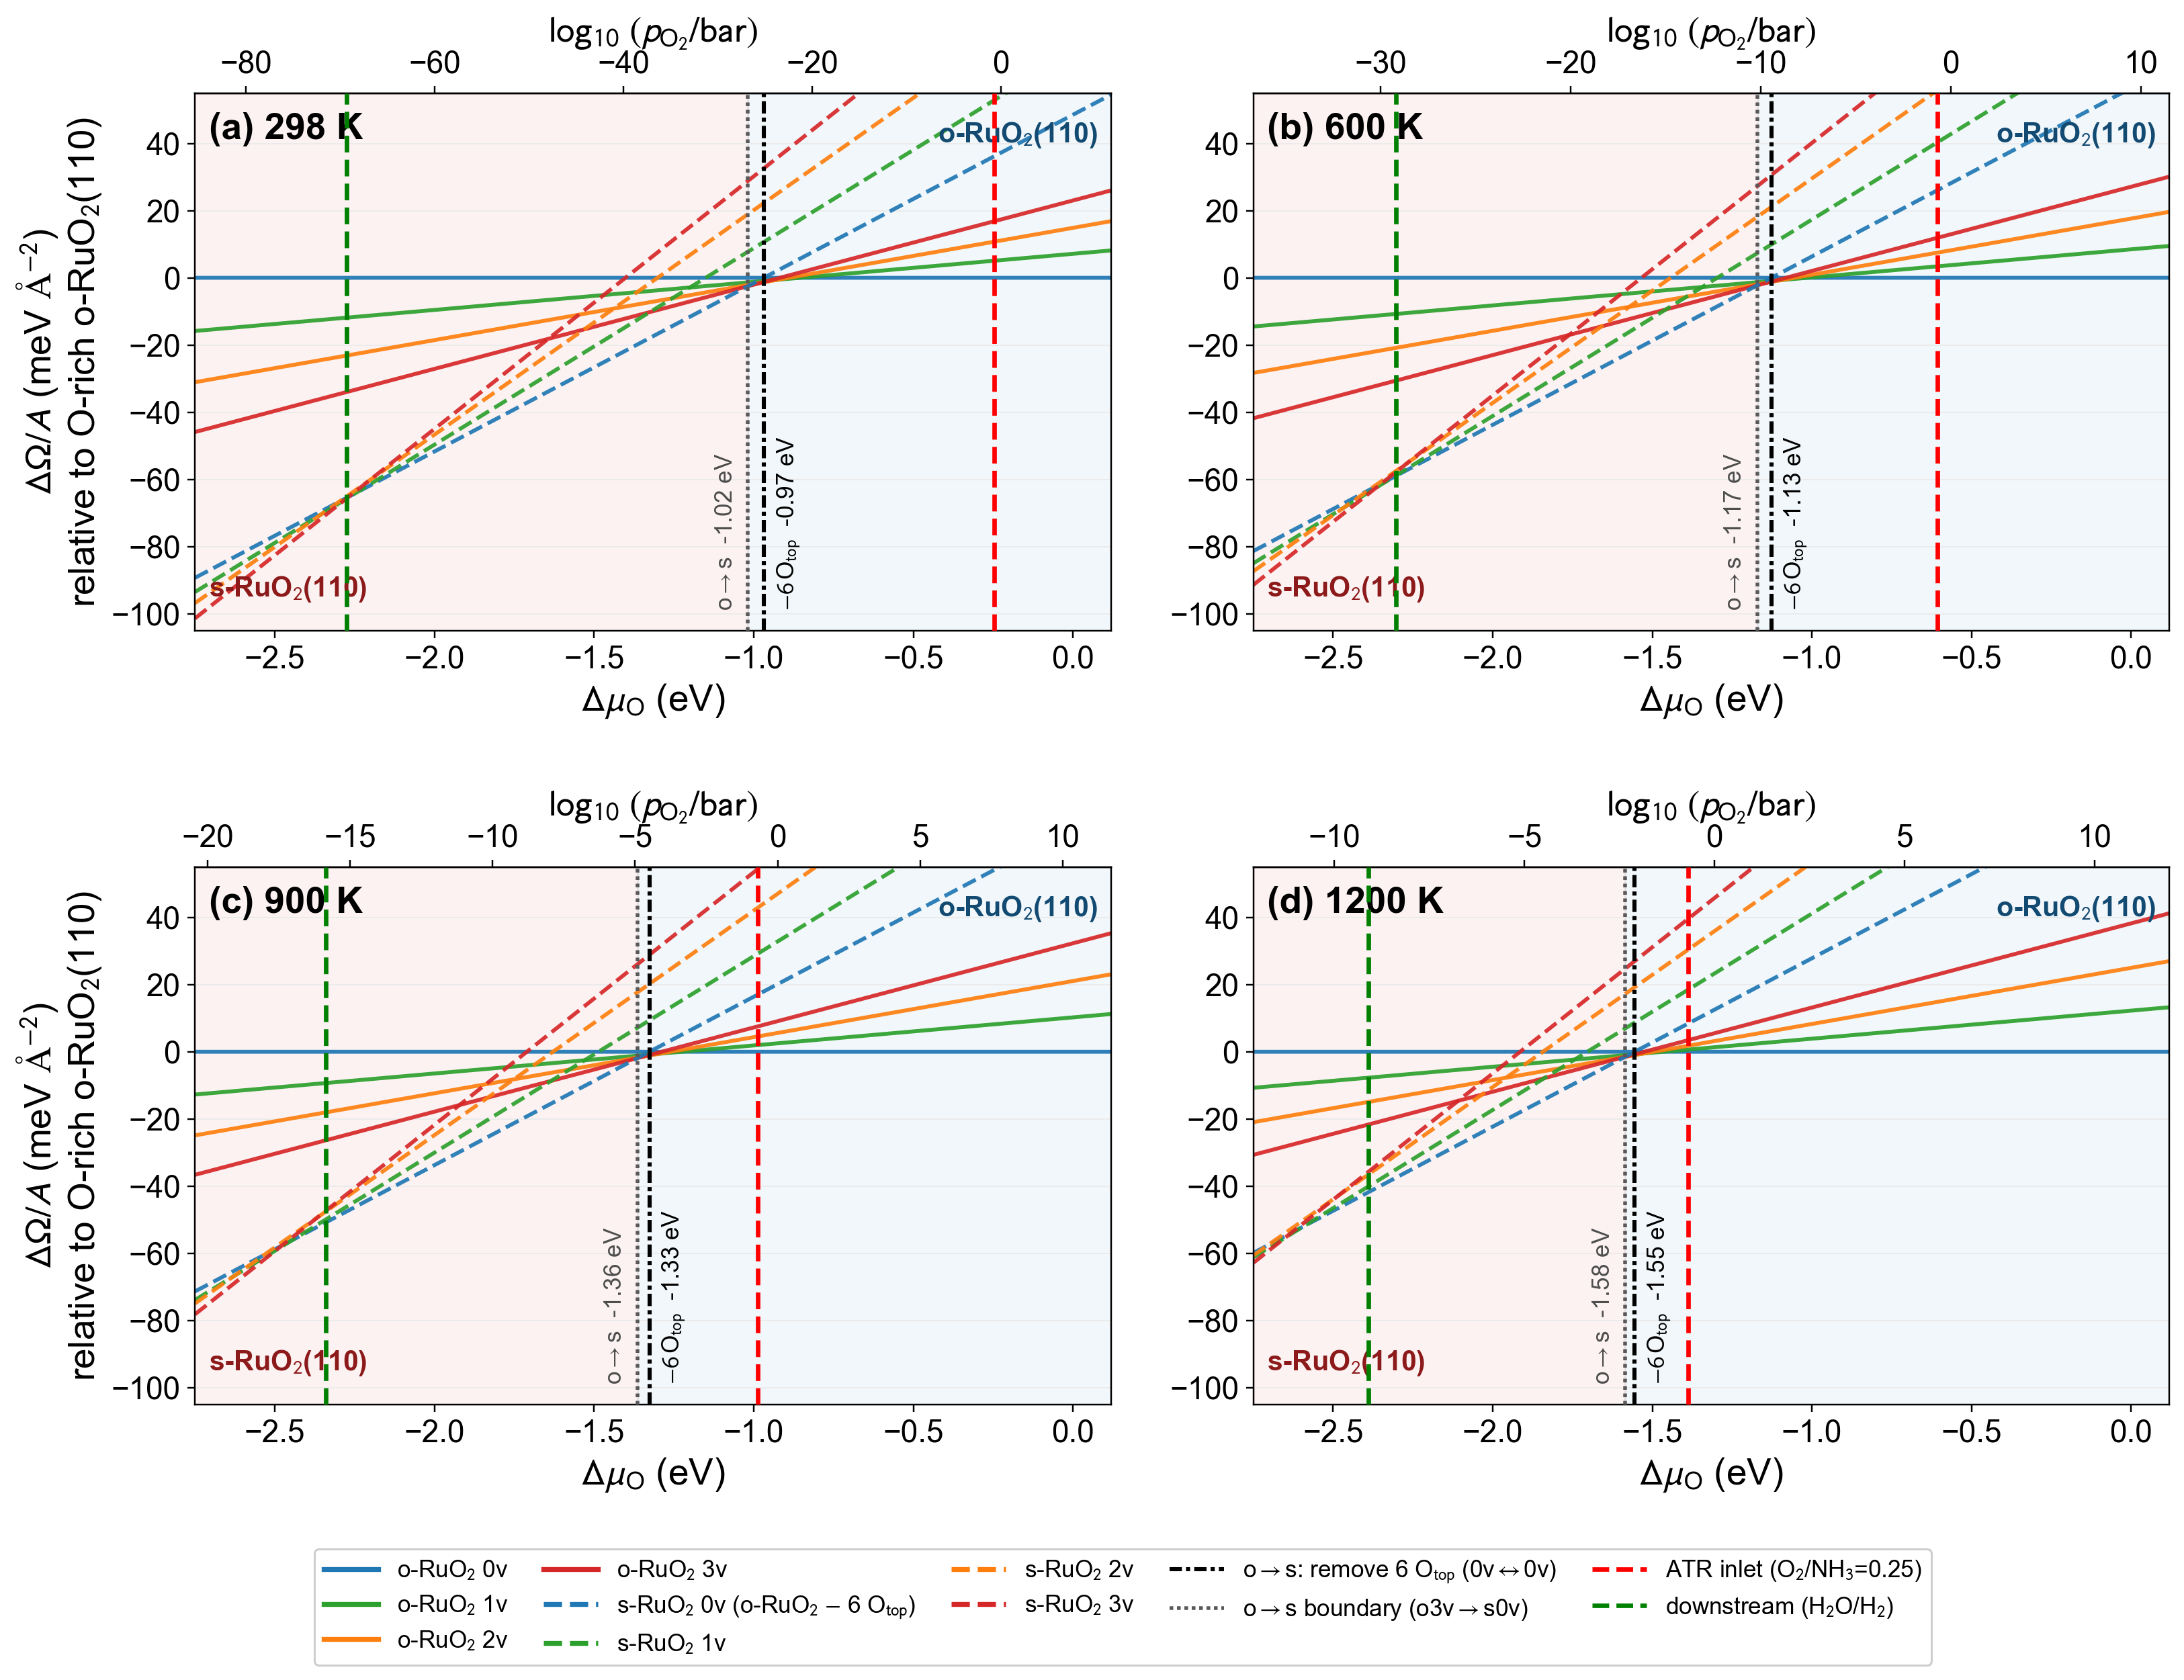
\includegraphics[width=\linewidth]{fig9_unified_states_2x2_dft.png}
  \caption{Relative surface grand potential $\Delta\Omega_k/A$ of the
  \textit{o}- and \textit{s}-RuO$_2$(110) terminations, all referenced to a single
  \textit{o}-RuO$_2$(110) 0v surface, at (a)~298, (b)~600, (c)~900 and (d)~1200~K.
  Solid lines, \textit{o}-RuO$_2$(110) $k$-vacancy surfaces (0--3v); dashed lines,
  \textit{s}-RuO$_2$(110) surfaces, with \textit{s}-RuO$_2$(110) 0v being
  \textit{o}-RuO$_2$(110) with its six on-top oxygens removed
  (Ru$_{36}$O$_{78}\rightarrow$Ru$_{36}$O$_{72}$). The black dash-dotted line marks
  the direct \textit{o}$\rightarrow$\textit{s} transition by removal of the six
  on-top oxygens (0v$\leftrightarrow$0v); the grey dotted line marks the
  \textit{o}$\rightarrow$\textit{s} transition between the most stable terminations
  (\textit{o}-RuO$_2$ 3v $\rightarrow$ \textit{s}-RuO$_2$ 0v). Red and green dashed verticals locate the
  ATR inlet ($\mathrm{O_2/NH_3}=0.25$) and downstream reforming
  ($\mathrm{H_2O/H_2}=10$) oxygen chemical potentials
  (Eqs.~\eqref{eq:inlet}--\eqref{eq:down}). Shaded bands indicate the
  \textit{s}-stable (left) and \textit{o}-stable (right) regions. The upper axis of
  each panel gives the corresponding oxygen partial pressure,
  $\log_{10}\!\left(p_{\mathrm{O_2}}/\mathrm{bar}\right)$ (Eq.~\eqref{eq:pO2}); all
  panels share a common axis.}
  \label{fig:unified}
\end{figure*}

\begin{figure*}[htbp]
  \centering
  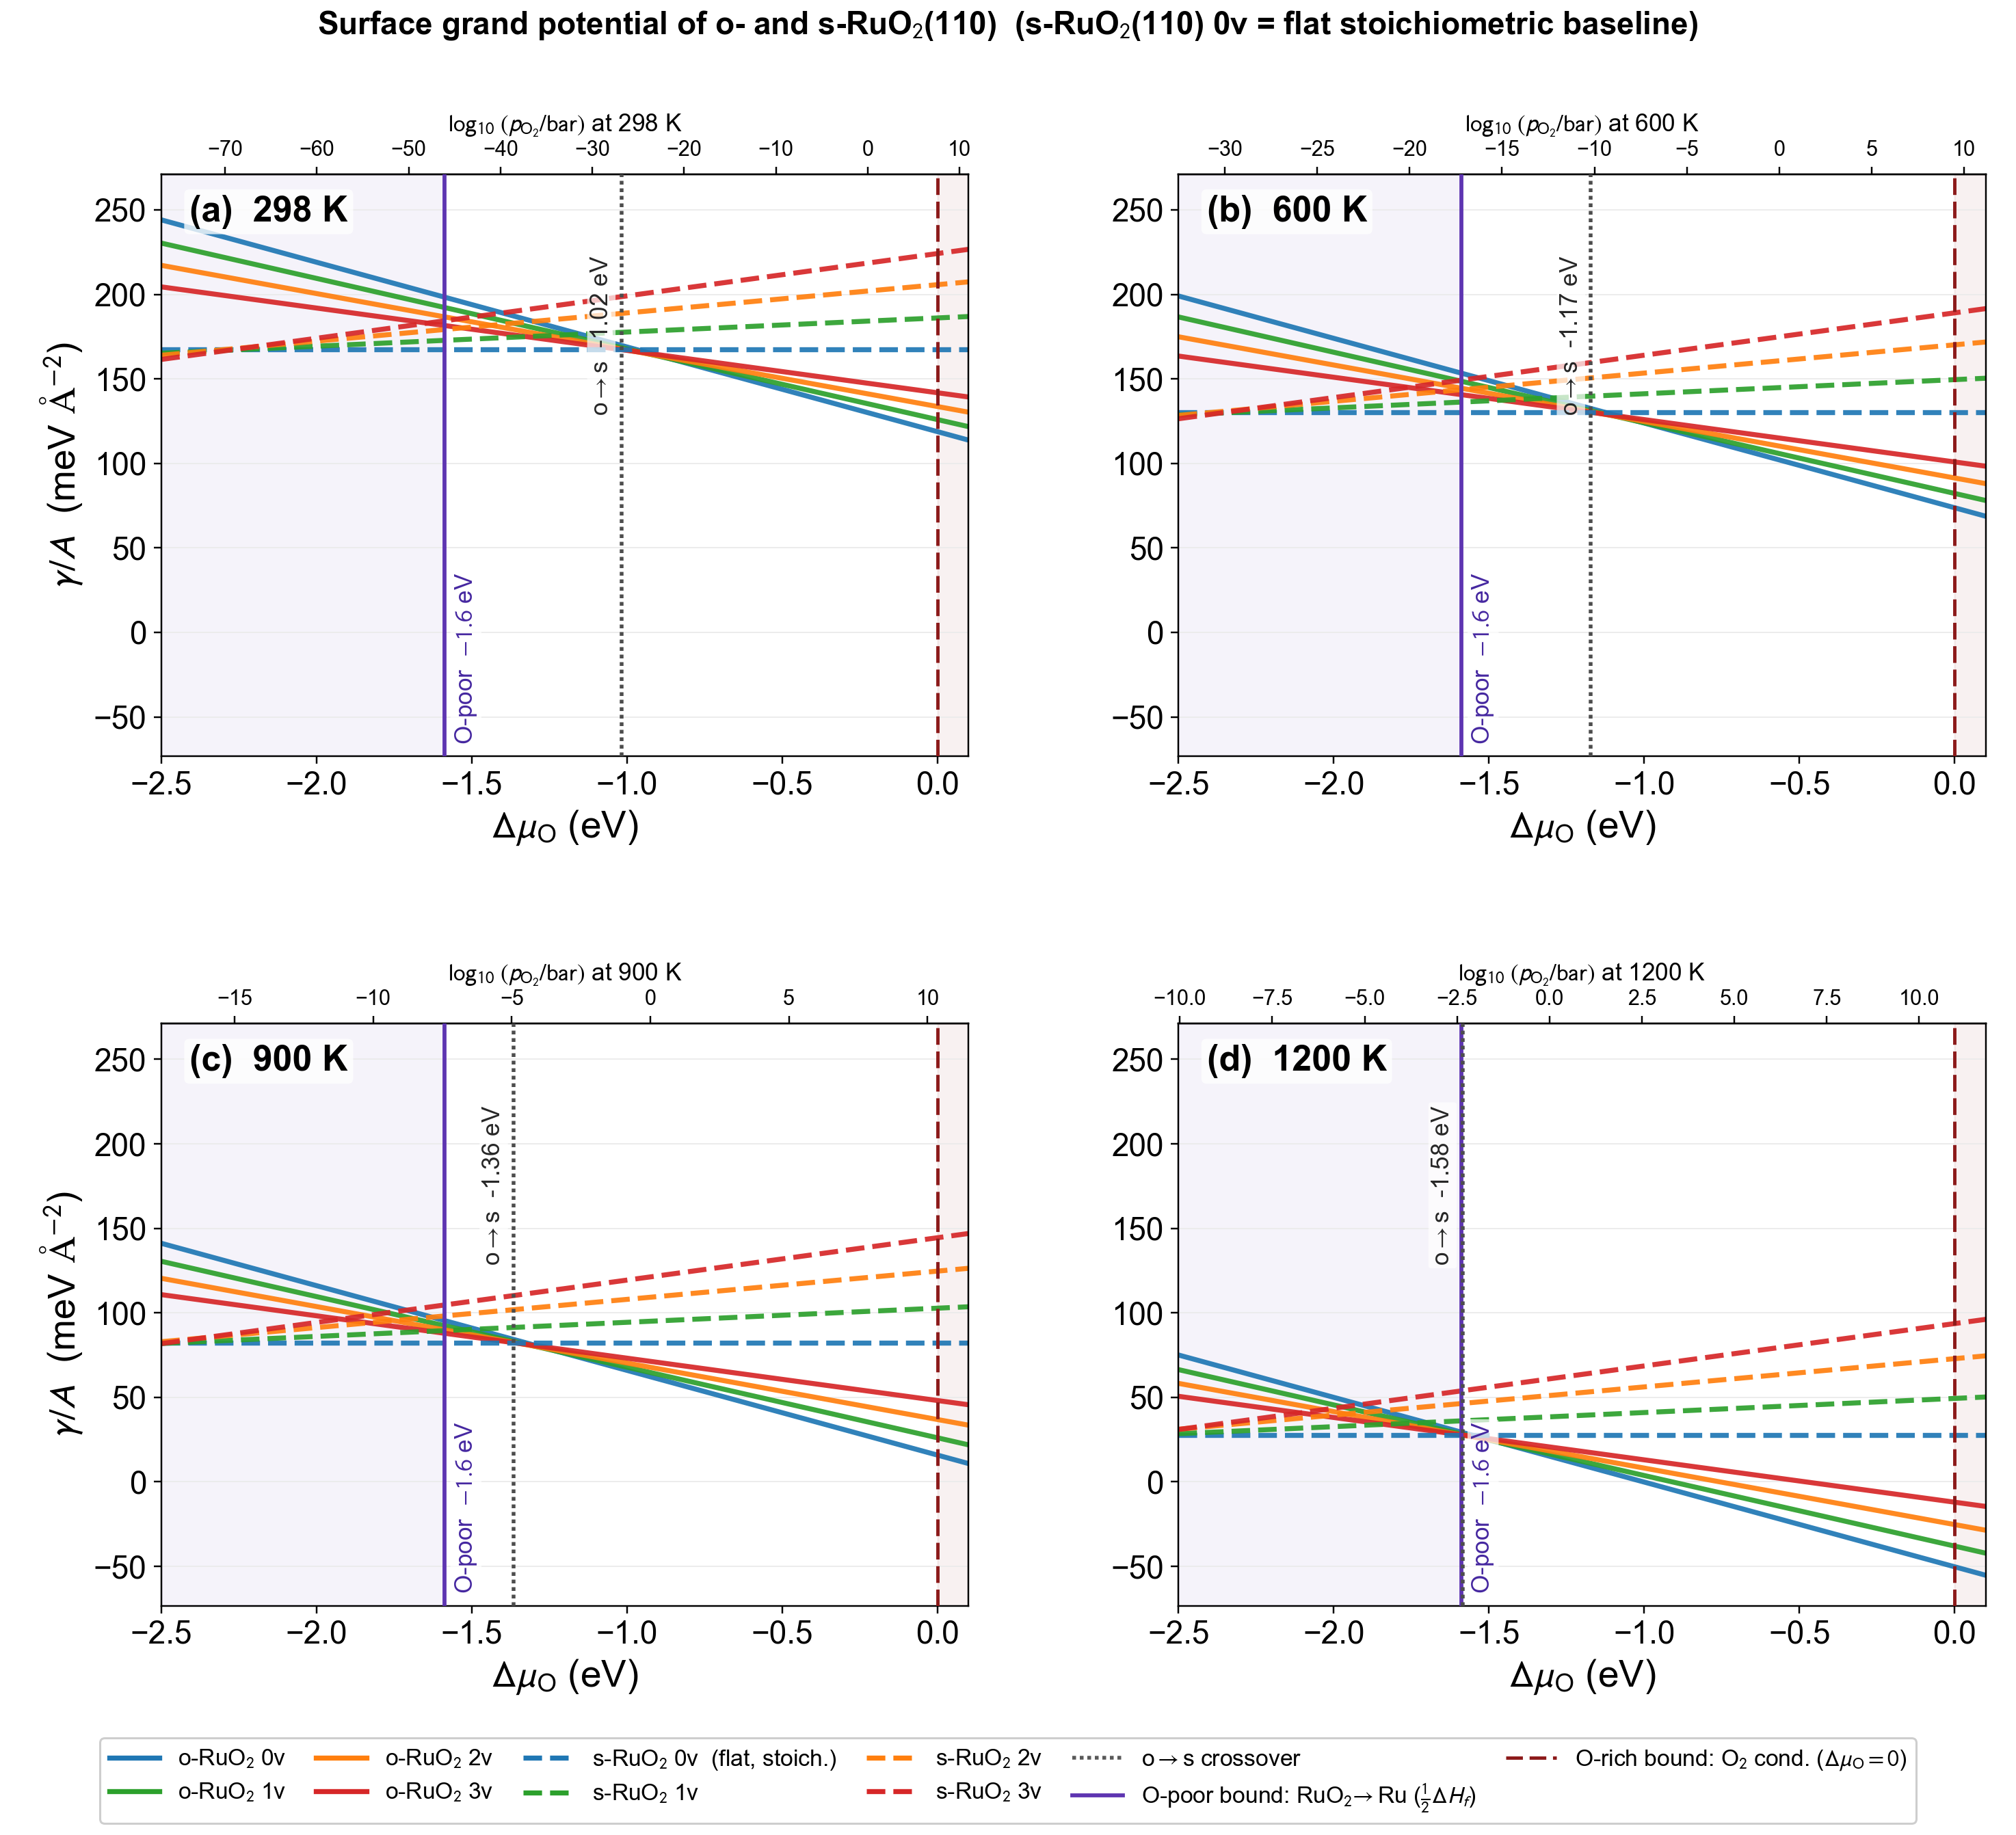
\includegraphics[width=\linewidth]{fig_bulk_referenced_2x2_dft.png}
  \caption{Surface grand potential of the \textit{o}- and
  \textit{s}-RuO$_2$(110) terminations referenced to bulk RuO$_2$ (absolute
  surface free energy $\gamma$) at (a)~298, (b)~600, (c)~900 and (d)~1200~K.
  Solid lines, \textit{o}-RuO$_2$(110) $k$-vacancy surfaces; dashed lines,
  \textit{s}-RuO$_2$(110); the stoichiometric \textit{s}-RuO$_2$(110) 0v surface
  is flat. The dotted line marks the \textit{o}$\rightarrow$\textit{s} boundary
  separating stable \textit{s}-RuO$_2$(110) (left) from \textit{o}-RuO$_2$(110)
  (right), identical to that of Figure~\ref{fig:unified}. Shaded bands are
  thermodynamically
  inaccessible: the oxygen-rich limit at $\Delta\mu_{\mathrm O}=0$ (O$_2$
  condensation) and the oxygen-poor limit at
  $\Delta\mu_{\mathrm O}=\tfrac{1}{2}\Delta H_f^{\,\mathrm{RuO_2}}\approx-1.60$~eV
  (decomposition to metallic Ru, Eq.~\eqref{eq:opoor}). The upper axis of each
  panel gives the corresponding oxygen partial pressure,
  $\log_{10}\!\left(p_{\mathrm{O_2}}/\mathrm{bar}\right)$, at that temperature
  (Eq.~\eqref{eq:pO2}). All panels share a common $\gamma$ axis.}
  \label{fig:bulkref}
\end{figure*}
  where this section
%  should appear (e.g. in the Supporting Information). Requires amsmath +
%  amssymb, which are already loaded in ATR NH3.tex.
%
%  FIGURE: the bulk-referenced grand-potential figure uses graphicx (already
%  loaded in ATR NH3.tex) and the image file fig_bulk_referenced_2x2_dft.png,
%  which is committed alongside this .tex at the project root.
%
%  OPTIONAL SI equation numbering (S11, S12, ...): add these two lines to
%  your PREAMBLE, before \begin{document}:
%     \renewcommand{\theequation}{S\arabic{equation}}
%     \setcounter{equation}{10}
%
%  NOTE (revtex twocolumn): the three wide displays (Svib, dOmega/A, log10)
%  can overflow a single column; wrap them in \begin{widetext}...\end{widetext}
%  or compile the SI in onecolumn if they run over.
% =====================================================================

\section*{Computational Details}

\subsection*{Electronic-structure calculations}
Spin-polarized density functional theory (DFT) calculations were performed with
the Perdew--Burke--Ernzerhof (PBE) exchange--correlation functional in the Vienna
\textit{Ab initio} Simulation Package (VASP), using the projector augmented-wave
method and a 430~eV plane-wave cutoff, as detailed in Section~2 of the main text.
The RuO$_2$(110) surfaces were modeled as $(2\times2)$ three-trilayer slabs and
the Ru(0001) surface as a $(4\times4)$ slab, each separated from its periodic
images by a vacuum gap.

\subsection*{Free-energy corrections}
The Gibbs free energy of every slab configuration used in the thermodynamic
analysis is evaluated from its DFT total energy $E_{\mathrm{DFT}}$ together with
the zero-point energy and vibrational (entropic) corrections obtained from the
harmonic vibrational frequencies $\nu_i$:
\begin{equation}
  G_{\mathrm{slab}}(T) = E_{\mathrm{DFT}} + E_{\mathrm{ZPE}}
  - T\,S_{\mathrm{vib}}(T)
  \label{eq:Gslab}
\end{equation}
\begin{equation}
  E_{\mathrm{ZPE}} = \tfrac{1}{2}\sum_i h\nu_i
  \label{eq:ZPE}
\end{equation}
\begin{equation}
  S_{\mathrm{vib}}(T) = k_{\mathrm B}\sum_i\left[
    \frac{h\nu_i/k_{\mathrm B}T}{e^{\,h\nu_i/k_{\mathrm B}T}-1}
    - \ln\!\left(1-e^{-h\nu_i/k_{\mathrm B}T}\right)\right]
  \label{eq:Svib}
\end{equation}
where $k_{\mathrm B}$ and $h$ are the Boltzmann and Planck constants. Because the
zero-point and vibrational-entropy terms are folded directly into
$G_{\mathrm{slab}}(T)$, the tabulated slab free energies are temperature
dependent (e.g., \textit{o}-RuO$_2$(110) 0v: $-817.70$~eV at $0$~K
$\rightarrow -837.48$~eV at $1200$~K), and no additional entropy term is applied
in the grand-potential expressions below. Vibrational frequencies of gas-phase
species were taken from the NIST Computational Chemistry Comparison and Benchmark
Database.

\subsection*{Oxygen reservoir chemical potential}
The surface exchanges lattice oxygen with a gas-phase O$_2$ reservoir. At
temperature $T$ and pressure $p$ the reservoir chemical potential varies with
pressure as
\begin{equation}
  \mu_{\mathrm{O_2}}(T,p) = \mu_{\mathrm{O_2}}(T,p^{0})
  + k_{\mathrm B}T\ln\!\left(p/p^{0}\right)
  \label{eq:muO2}
\end{equation}
and the oxygen chemical potential is one-half of it, referenced to the $0$~K DFT
O$_2$ energy:
\begin{equation}
  \mu_{\mathrm O}(T,p) = \tfrac{1}{2}\mu_{\mathrm{O_2}}(T,p)
  = \tfrac{1}{2}G_{\mathrm{O_2}}(0\,\mathrm{K}) + \Delta\mu_{\mathrm O}
  \label{eq:muO}
\end{equation}
\begin{equation}
  \Delta\mu_{\mathrm O} =
  \tfrac{1}{2}\left[G_{\mathrm{O_2}}(T) - G_{\mathrm{O_2}}(0\,\mathrm{K})\right]
  + \tfrac{1}{2}k_{\mathrm B}T\ln\!\left(p_{\mathrm{O_2}}/p^{0}\right)
  \label{eq:dmuO}
\end{equation}
so that $\Delta\mu_{\mathrm O}=0$ corresponds to gas-phase O$_2$ at $0$~K and more
negative $\Delta\mu_{\mathrm O}$ denotes more reducing conditions. The thermal term
$\tfrac{1}{2}[G_{\mathrm{O_2}}(T)-G_{\mathrm{O_2}}(0\,\mathrm{K})]$ is evaluated
directly from our calculated ideal-gas Gibbs free energy of O$_2$ (translational,
rotational, and vibrational contributions), giving $-0.23$, $-0.57$, $-0.93$, and
$-1.31$~eV per O atom at $298$, $600$, $900$, and $1200$~K, respectively.

\subsection*{Surface grand potential}
The grand potential of a slab open to the oxygen reservoir is
\begin{equation}
  \Omega = U - T\,S(T) - \sum_i \mu_i N_i
  \label{eq:Omega_gen}
\end{equation}
Using the slab free energy of Eq.~\eqref{eq:Gslab} for the $U-TS$ term and noting
that only oxygen is exchanged with the reservoir while ruthenium is conserved,
this becomes
\begin{equation}
  \Omega = G_{\mathrm{slab}}(T) - \mu_{\mathrm O} N_{\mathrm O}
  - \mu_{\mathrm{Ru}} N_{\mathrm{Ru}}
  \label{eq:Omega_surf}
\end{equation}
where $N_{\mathrm O}$ and $N_{\mathrm{Ru}}$ are the numbers of O and Ru atoms in
the cell. Because every termination contains the same $N_{\mathrm{Ru}}=36$, the
$\mu_{\mathrm{Ru}}N_{\mathrm{Ru}}$ term is identical across surfaces and cancels
when grand potentials are compared.

\subsection*{Relative (referenced) grand potential}
Terminations are compared through the grand potential of each $k$-vacancy surface
relative to a vacancy-free reference, per unit surface area $A$
($=119.70~\text{\AA}^{2}$ for the $(2\times2)$ cell):
\begin{equation}
  \frac{\Delta\Omega_k}{A} =
  \frac{\left[G_{\mathrm{slab}}^{(k)}(T)
  - G_{\mathrm{slab}}^{(\mathrm{ref})}(T)\right]
  + n_{\mathrm{vac}}\left(\tfrac{1}{2}G_{\mathrm{O_2}}(0\,\mathrm{K})
  + \Delta\mu_{\mathrm O}\right)}{A}
  \label{eq:dOmega}
\end{equation}
where $n_{\mathrm{vac}} = N_{\mathrm O}^{(\mathrm{ref})} - N_{\mathrm O}^{(k)}$ is
the number of oxygen atoms removed relative to the reference, so the slope of each
line, $n_{\mathrm{vac}}/A$, is the areal density of released oxygen. The
referencing subtracts a common term ($\mu_{\mathrm{Ru}}N_{\mathrm{Ru}}$ and the
bulk contribution), making $\Delta\Omega$ independent of the ruthenium reference.
This relative construction is thermodynamically equivalent to the absolute surface
free energy $\gamma = (1/A)[\,G_{\mathrm{slab}} - N_{\mathrm{Ru}}\,g^{\mathrm{bulk}}_{\mathrm{RuO_2}}
- (N_{\mathrm O}-2N_{\mathrm{Ru}})\,\mu_{\mathrm O}\,]$ of Reuter and Scheffler
[K.~Reuter and M.~Scheffler, Phys.\ Rev.\ B \textbf{65}, 035406 (2001)]: because
every termination shares the same $N_{\mathrm{Ru}}$, referencing to the
\textit{o}-RuO$_2$(110) 0v surface removes the $\mu_{\mathrm{Ru}}$ term by
construction, instead of through the bulk-equilibrium constraint
$\mu_{\mathrm{Ru}}+2\mu_{\mathrm O}=g^{\mathrm{bulk}}_{\mathrm{RuO_2}}$ that references
$\gamma$ to bulk RuO$_2$; both choices leave every crossover and vacancy-formation
threshold unchanged.
This unified construction is shown in Figure~\ref{fig:unified}, in which all
terminations share the single \textit{o}-RuO$_2$(110) 0v reference, using the fact
that \textit{s}-RuO$_2$(110) 0v is \textit{o}-RuO$_2$(110) with its six on-top
oxygens removed (Ru$_{36}$O$_{78} \rightarrow$ Ru$_{36}$O$_{72}$,
$n_{\mathrm{vac}}=6$). The equivalent diagram referenced to bulk RuO$_2$ is shown
in Figure~\ref{fig:bulkref}; presenting the two reference choices side by side
demonstrates that the \textit{o}$\rightarrow$\textit{s} crossover and
vacancy-formation thresholds are independent of the reference.

\subsection*{Operating oxygen chemical potentials}
The ATR inlet is set by a fixed feed oxygen partial pressure
(O$_2$/NH$_3 = 0.25 \rightarrow p_{\mathrm{O_2}} = 0.2$~bar):
\begin{equation}
  \Delta\mu_{\mathrm O}^{\,\mathrm{inlet}} =
  \tfrac{1}{2}\left[G_{\mathrm{O_2}}(T) - G_{\mathrm{O_2}}(0\,\mathrm{K})\right]
  + \tfrac{1}{2}k_{\mathrm B}T\ln\!\left(p_{\mathrm{O_2}}/p^{0}\right)
  \label{eq:inlet}
\end{equation}
The downstream reforming potential is fixed by the
H$_2 + \tfrac{1}{2}$O$_2 \rightleftharpoons$ H$_2$O equilibrium, and is
independent of the O$_2$ reference:
\begin{equation}
  \Delta\mu_{\mathrm O}^{\,\mathrm{down}} =
  \left[G_{\mathrm{H_2O}}(T) - G_{\mathrm{H_2}}(T)\right]
  - \tfrac{1}{2}G_{\mathrm{O_2}}(0\,\mathrm{K})
  + k_{\mathrm B}T\ln\!\left(p_{\mathrm{H_2O}}/p_{\mathrm{H_2}}\right)
  \label{eq:down}
\end{equation}
evaluated at $p_{\mathrm{H_2O}}/p_{\mathrm{H_2}}=10$. The upper axes of
Figures~\ref{fig:unified} and~\ref{fig:bulkref} convert $\Delta\mu_{\mathrm O}$
into an equivalent O$_2$ partial pressure by
inverting Eq.~\eqref{eq:dmuO}:
\begin{equation}
  \log_{10}\!\left(p_{\mathrm{O_2}}/p^{0}\right) =
  \frac{\Delta\mu_{\mathrm O}
  - \tfrac{1}{2}\left(G_{\mathrm{O_2}}(T) - G_{\mathrm{O_2}}(0\,\mathrm{K})\right)}
       {\tfrac{1}{2}k_{\mathrm B}T\ln 10}
  \label{eq:pO2}
\end{equation}
with $p^{0}=1$~bar the standard-state pressure.

\subsection*{Bulk-referenced surface stability and correlation to ATR conditions}
Referencing the surface grand potential to bulk RuO$_2$ rather than to the
\textit{o}-RuO$_2$(110) 0v surface converts the relative curves of
Eq.~\eqref{eq:dOmega} into absolute surface free energies
$\gamma(\Delta\mu_{\mathrm O})$ and, in addition, places the accessible oxygen
chemical potential on a physical scale bounded by two limits. The oxygen-rich
limit is fixed by O$_2$ condensation, $\Delta\mu_{\mathrm O}=0$; the oxygen-poor
limit is fixed by decomposition of the oxide into metallic ruthenium,
$\mathrm{RuO_2}\rightarrow\mathrm{Ru}+\mathrm{O_2}$, which occurs when
\begin{equation}
  \Delta\mu_{\mathrm O}^{\,\mathrm{poor}} =
  \tfrac{1}{2}\,\Delta H_f^{\,\mathrm{RuO_2}} \approx -1.60~\mathrm{eV},
  \label{eq:opoor}
\end{equation}
using the experimental heat of formation $\Delta H_f^{\,\mathrm{RuO_2}}=-3.19$~eV
[NIST--JANAF; consistent with the value adopted by Reuter and Scheffler,
Phys.\ Rev.\ B \textbf{68}, 045407 (2003)]. Because $\Delta\mu_{\mathrm O}$
already carries the full temperature and pressure dependence of the O$_2$
reservoir (Eq.~\eqref{eq:dmuO}), this decomposition bound is temperature
independent. Figure~\ref{fig:bulkref} shows the resulting diagram at 298, 600,
900 and 1200~K. In this reference the stoichiometric \textit{s}-RuO$_2$(110) 0v
surface ($N_{\mathrm O}=2N_{\mathrm{Ru}}$) is flat, whereas every oxygen-rich
termination slopes downward with a slope equal to its excess-oxygen areal
density, $-(N_{\mathrm O}-2N_{\mathrm{Ru}})/A$
($-50.1$~meV\,\AA$^{-2}$\,eV$^{-1}$ for the six on-top oxygens of
\textit{o}-RuO$_2$(110) 0v). Every \textit{o}$\rightarrow$\textit{s} crossover is
numerically identical to that of the \textit{o}-RuO$_2$(110)-referenced diagram
(Figure~\ref{fig:unified}), confirming that the surface phase
boundaries are independent of the chosen reference.

At any oxygen potential the thermodynamically stable surface is simply the
termination of lowest $\gamma$. On the oxygen-rich (right) side of each panel this
is the steeply sloped, oxygen-covered \textit{o}-RuO$_2$(110) surface; on the
oxygen-poor (left) side it is the flat stoichiometric \textit{s}-RuO$_2$(110)
0v surface. The dotted vertical line marks the oxygen potential at which the two are
equally stable---the \textit{o}$\rightarrow$\textit{s} boundary---at
$\Delta\mu_{\mathrm O}=-1.02$, $-1.17$, $-1.36$ and $-1.58$~eV for 298, 600, 900
and 1200~K, respectively. To the right of this line the oxidised
\textit{o}-RuO$_2$(110) surface is stable; to the left, the surface has released its
on-top oxygens to become the reduced \textit{s}-RuO$_2$(110) termination. The closer
an operating point sits to this boundary, the smaller the free-energy margin (a few
meV\,\AA$^{-2}$) between the two terminations, so near it the oxidised and reduced
surfaces are effectively degenerate within DFT accuracy.

Superimposing the ATR operating potentials of
Eqs.~\eqref{eq:inlet}--\eqref{eq:down} on this stability window links the surface
oxidation state directly to reactor position. At the ATR inlet
($\mathrm{O_2/NH_3}=0.25$, $p_{\mathrm{O_2}}=0.2$~bar) the oxygen potential
$\Delta\mu_{\mathrm O}^{\,\mathrm{inlet}}$ ranges from $-0.25$~eV at 298~K to
$-1.39$~eV at 1200~K; it lies inside the RuO$_2$ stability window at every
temperature and on the oxygen-rich side of the
\textit{o}$\rightarrow$\textit{s} crossover, so the inlet surface is the
oxygen-covered \textit{o}-RuO$_2$(110) termination. Downstream, once the
$\mathrm{H_2O/H_2}$ reforming equilibrium is established
($\Delta\mu_{\mathrm O}^{\,\mathrm{down}}\approx-2.3$~eV at
$p_{\mathrm{H_2O}}/p_{\mathrm{H_2}}=10$), the potential falls \emph{below} the
oxide-decomposition bound of Eq.~\eqref{eq:opoor} at all temperatures: the
reducing reforming atmosphere drives the termination through the
\textit{s}-RuO$_2$(110) surface and ultimately toward metallic ruthenium. The
\textit{o}$\rightarrow$\textit{s} crossover ($-1.02$ to $-1.58$~eV) sits between
these two operating points, so a catalyst particle necessarily evolves from the
selective, oxygen-rich \textit{o}-RuO$_2$ surface near the inlet to the reduced
\textit{s}-RuO$_2$ surface as ammonia is consumed and the local gas becomes
reducing. Increasing temperature compresses this window: at 1200~K the inlet
potential ($-1.39$~eV), the \textit{o}$\rightarrow$\textit{s} crossover
($-1.58$~eV) and the decomposition bound ($-1.60$~eV) nearly coincide, so the
reduced surface---and eventually metallic Ru---becomes accessible even close to
the inlet, consistent with the loss of N$_2$ selectivity observed at high
temperature.

Reading these transitions on the equivalent oxygen-pressure scale (upper axes of
Figure~\ref{fig:bulkref}, Eq.~\eqref{eq:pO2}) makes the reactor gradient
explicit. Table~\ref{tab:po2markers} lists the oxygen partial pressure
$p_{\mathrm{O_2}}$ at the inlet, at the \textit{o}$\rightarrow$\textit{s}
crossover, at the oxide-decomposition bound and at the downstream reforming
point. As O$_2$ is consumed along the bed the local oxygen potential sweeps
monotonically toward lower $p_{\mathrm{O_2}}$, so a catalyst particle crosses
these markers in sequence: the oxygen-covered \textit{o}-RuO$_2$(110)
termination at the inlet, the \textit{o}$\rightarrow$\textit{s} transition once
$p_{\mathrm{O_2}}$ has dropped by the margin listed in the final column, and
finally reduction past the decomposition bound in the reforming zone. This
oxidative margin collapses from $\sim$26 orders of magnitude in
$p_{\mathrm{O_2}}$ at 298~K to only $\sim$1.7 at 1200~K, where the crossover and
the decomposition bound become numerically coincident
($p_{\mathrm{O_2}}\approx10^{-2.4}$~bar). The oxygen-covered, N$_2$-selective
surface therefore persists over essentially the entire bed at low temperature
but is confined to a thin zone near the inlet at high temperature, providing a
thermodynamic rationale for the loss of N$_2$ selectivity as temperature
increases.

\begin{table*}[htbp]
  \centering
  \caption{Equivalent oxygen partial pressure $p_{\mathrm{O_2}}$ (bar) at the
  ATR inlet, the \textit{o}$\rightarrow$\textit{s} crossover, the oxygen-poor
  (decomposition) bound and the downstream reforming point, obtained from the
  operating potentials (Eqs.~\eqref{eq:inlet}--\eqref{eq:down}) through
  Eq.~\eqref{eq:pO2}. The final column is the oxidative margin: the drop in
  $p_{\mathrm{O_2}}$ (orders of magnitude) between the inlet and the
  \textit{o}$\rightarrow$\textit{s} crossover.}
  \label{tab:po2markers}
  \begin{tabular}{cccccc}
    \hline
    $T$ (K) & inlet & \textit{o}$\rightarrow$\textit{s} &
    O-poor ($\rightarrow$Ru) & downstream &
    inlet$\rightarrow$\,\textit{o}$\rightarrow$\textit{s} \\
     & (bar) & (bar) & (bar) & (bar) & (decades) \\
    \hline
    298  & $0.2$ & $10^{-27}$  & $10^{-46}$  & $10^{-69}$  & 26  \\
    600  & $0.2$ & $10^{-10}$  & $10^{-17}$  & $10^{-29}$  & 9.5 \\
    900  & $0.2$ & $10^{-4.9}$ & $10^{-7.5}$ & $10^{-16}$  & 4.2 \\
    1200 & $0.2$ & $10^{-2.4}$ & $10^{-2.4}$ & $10^{-9.1}$ & 1.7 \\
    \hline
  \end{tabular}
\end{table*}

\begin{figure*}[htbp]
  \centering
  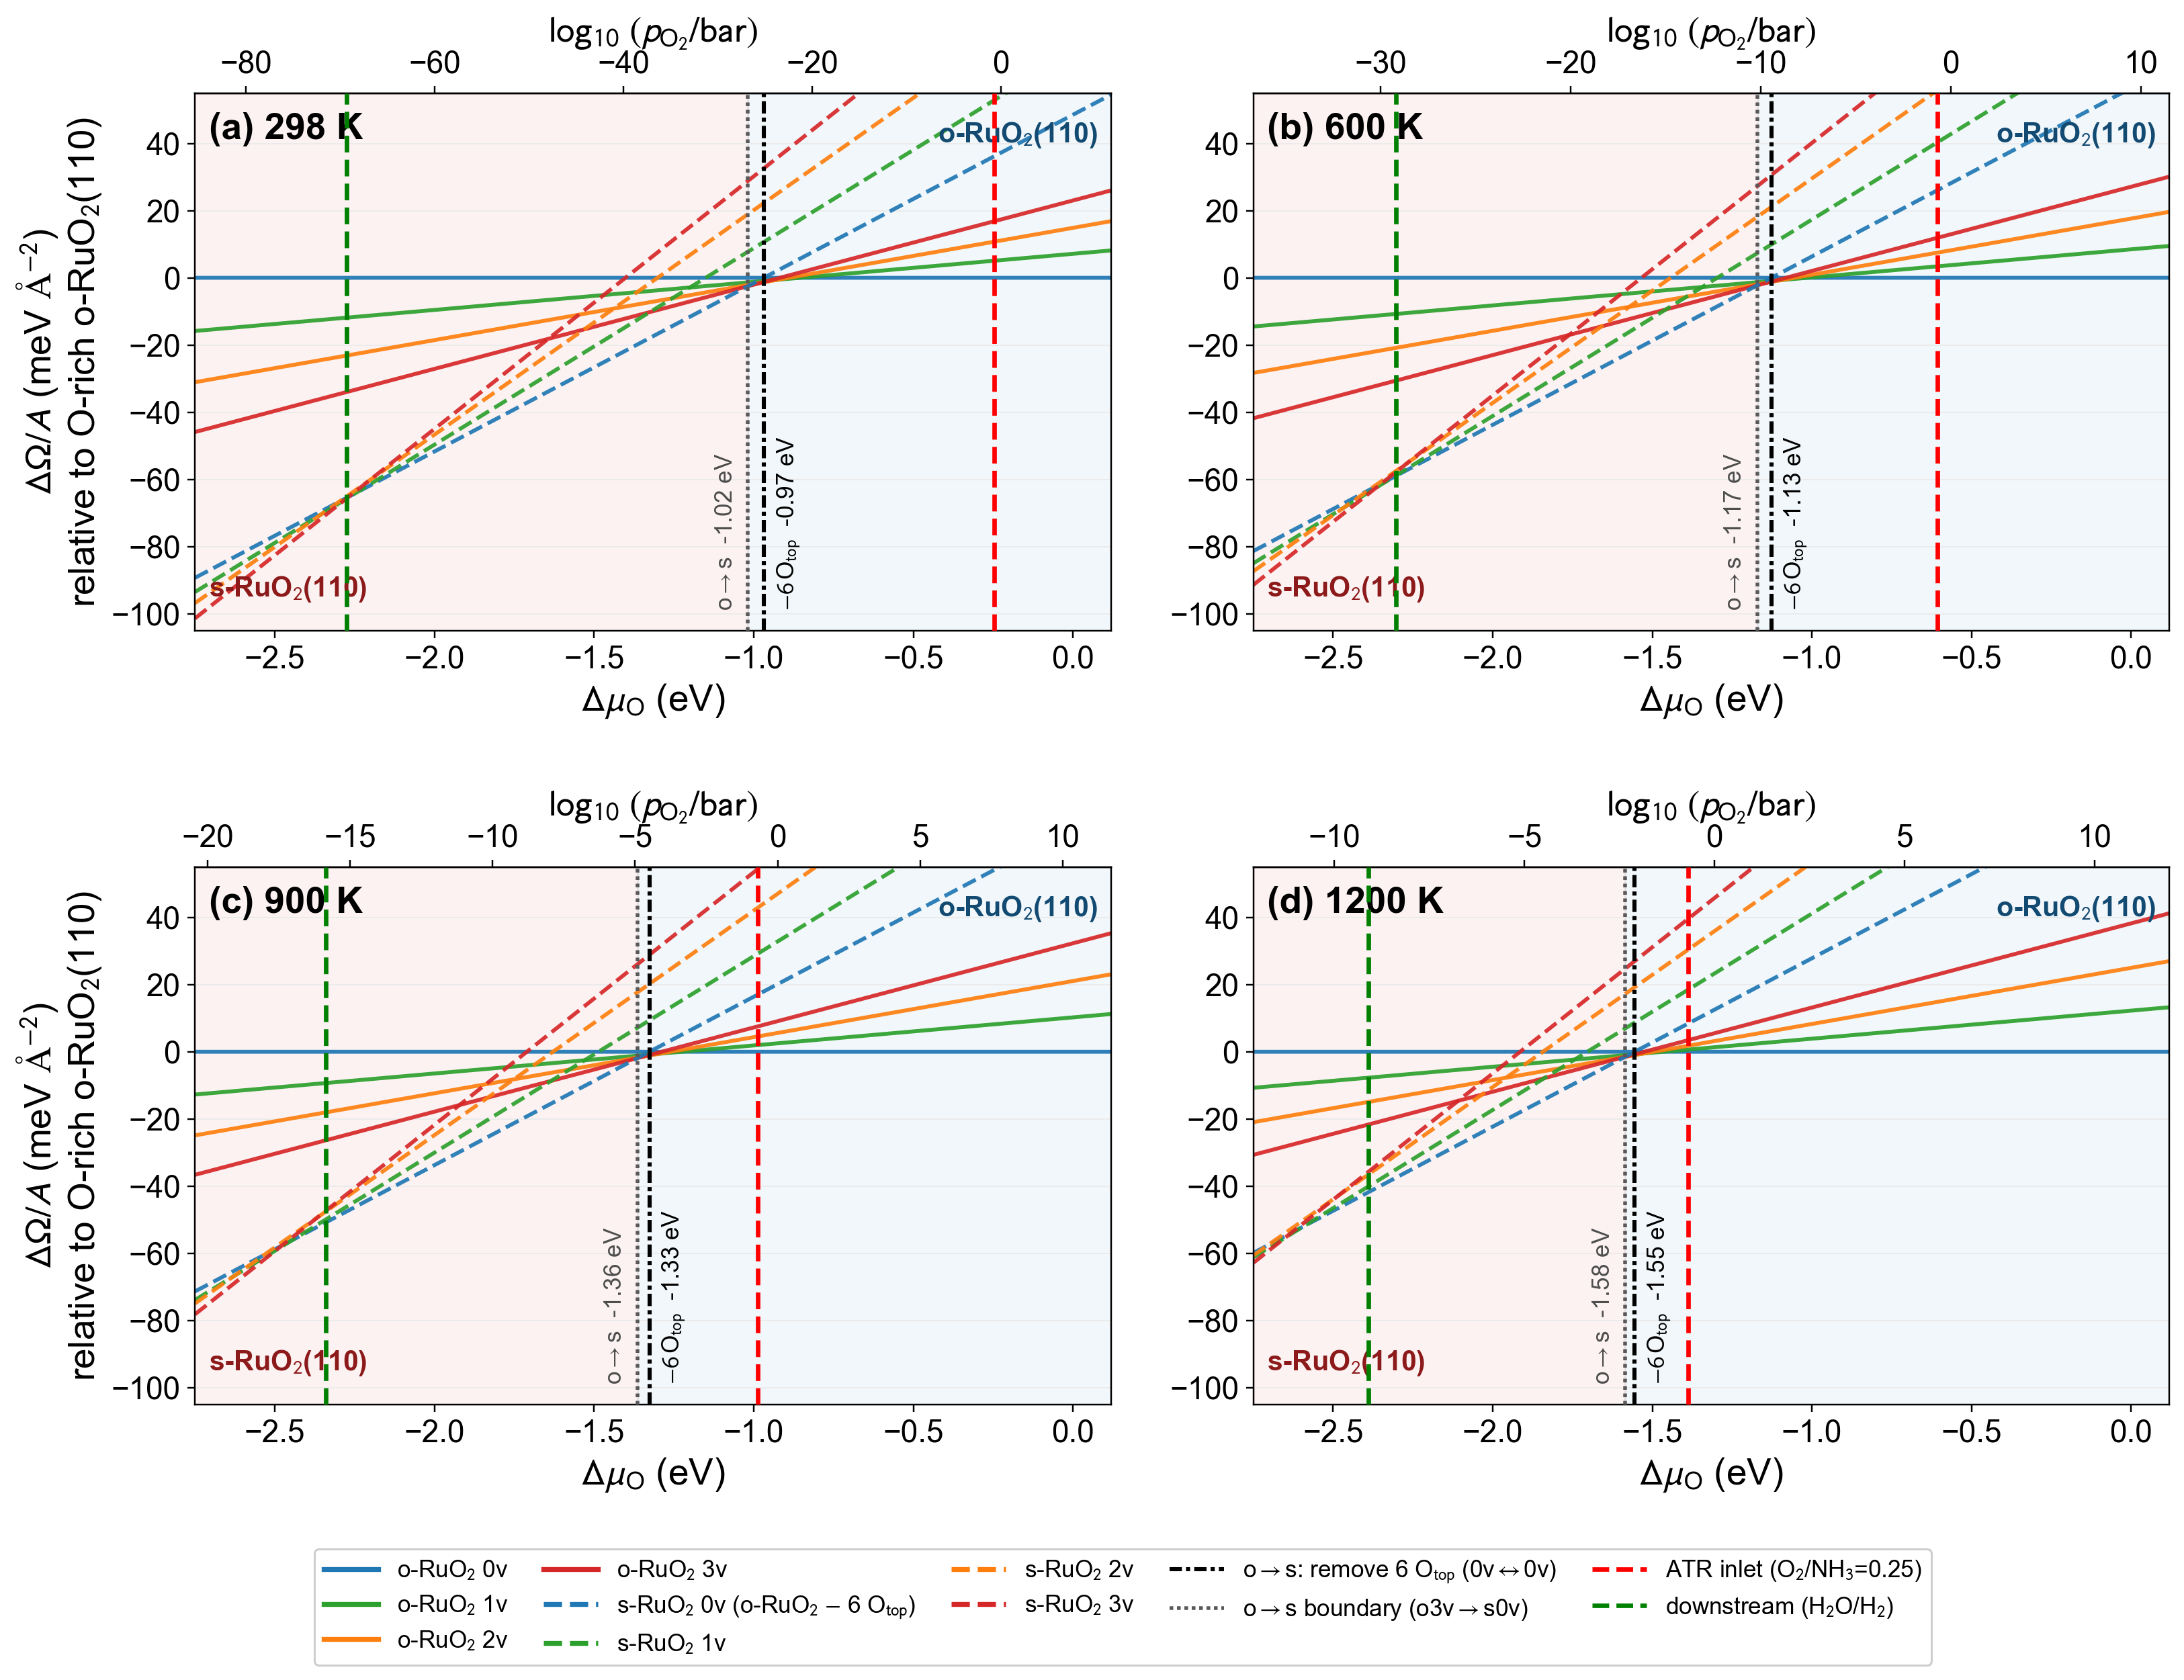
\includegraphics[width=\linewidth]{fig9_unified_states_2x2_dft.png}
  \caption{Relative surface grand potential $\Delta\Omega_k/A$ of the
  \textit{o}- and \textit{s}-RuO$_2$(110) terminations, all referenced to a single
  \textit{o}-RuO$_2$(110) 0v surface, at (a)~298, (b)~600, (c)~900 and (d)~1200~K.
  Solid lines, \textit{o}-RuO$_2$(110) $k$-vacancy surfaces (0--3v); dashed lines,
  \textit{s}-RuO$_2$(110) surfaces, with \textit{s}-RuO$_2$(110) 0v being
  \textit{o}-RuO$_2$(110) with its six on-top oxygens removed
  (Ru$_{36}$O$_{78}\rightarrow$Ru$_{36}$O$_{72}$). The black dash-dotted line marks
  the direct \textit{o}$\rightarrow$\textit{s} transition by removal of the six
  on-top oxygens (0v$\leftrightarrow$0v); the grey dotted line marks the
  \textit{o}$\rightarrow$\textit{s} transition between the most stable terminations
  (\textit{o}-RuO$_2$ 3v $\rightarrow$ \textit{s}-RuO$_2$ 0v). Red and green dashed verticals locate the
  ATR inlet ($\mathrm{O_2/NH_3}=0.25$) and downstream reforming
  ($\mathrm{H_2O/H_2}=10$) oxygen chemical potentials
  (Eqs.~\eqref{eq:inlet}--\eqref{eq:down}). Shaded bands indicate the
  \textit{s}-stable (left) and \textit{o}-stable (right) regions. The upper axis of
  each panel gives the corresponding oxygen partial pressure,
  $\log_{10}\!\left(p_{\mathrm{O_2}}/\mathrm{bar}\right)$ (Eq.~\eqref{eq:pO2}); all
  panels share a common axis.}
  \label{fig:unified}
\end{figure*}

\begin{figure*}[htbp]
  \centering
  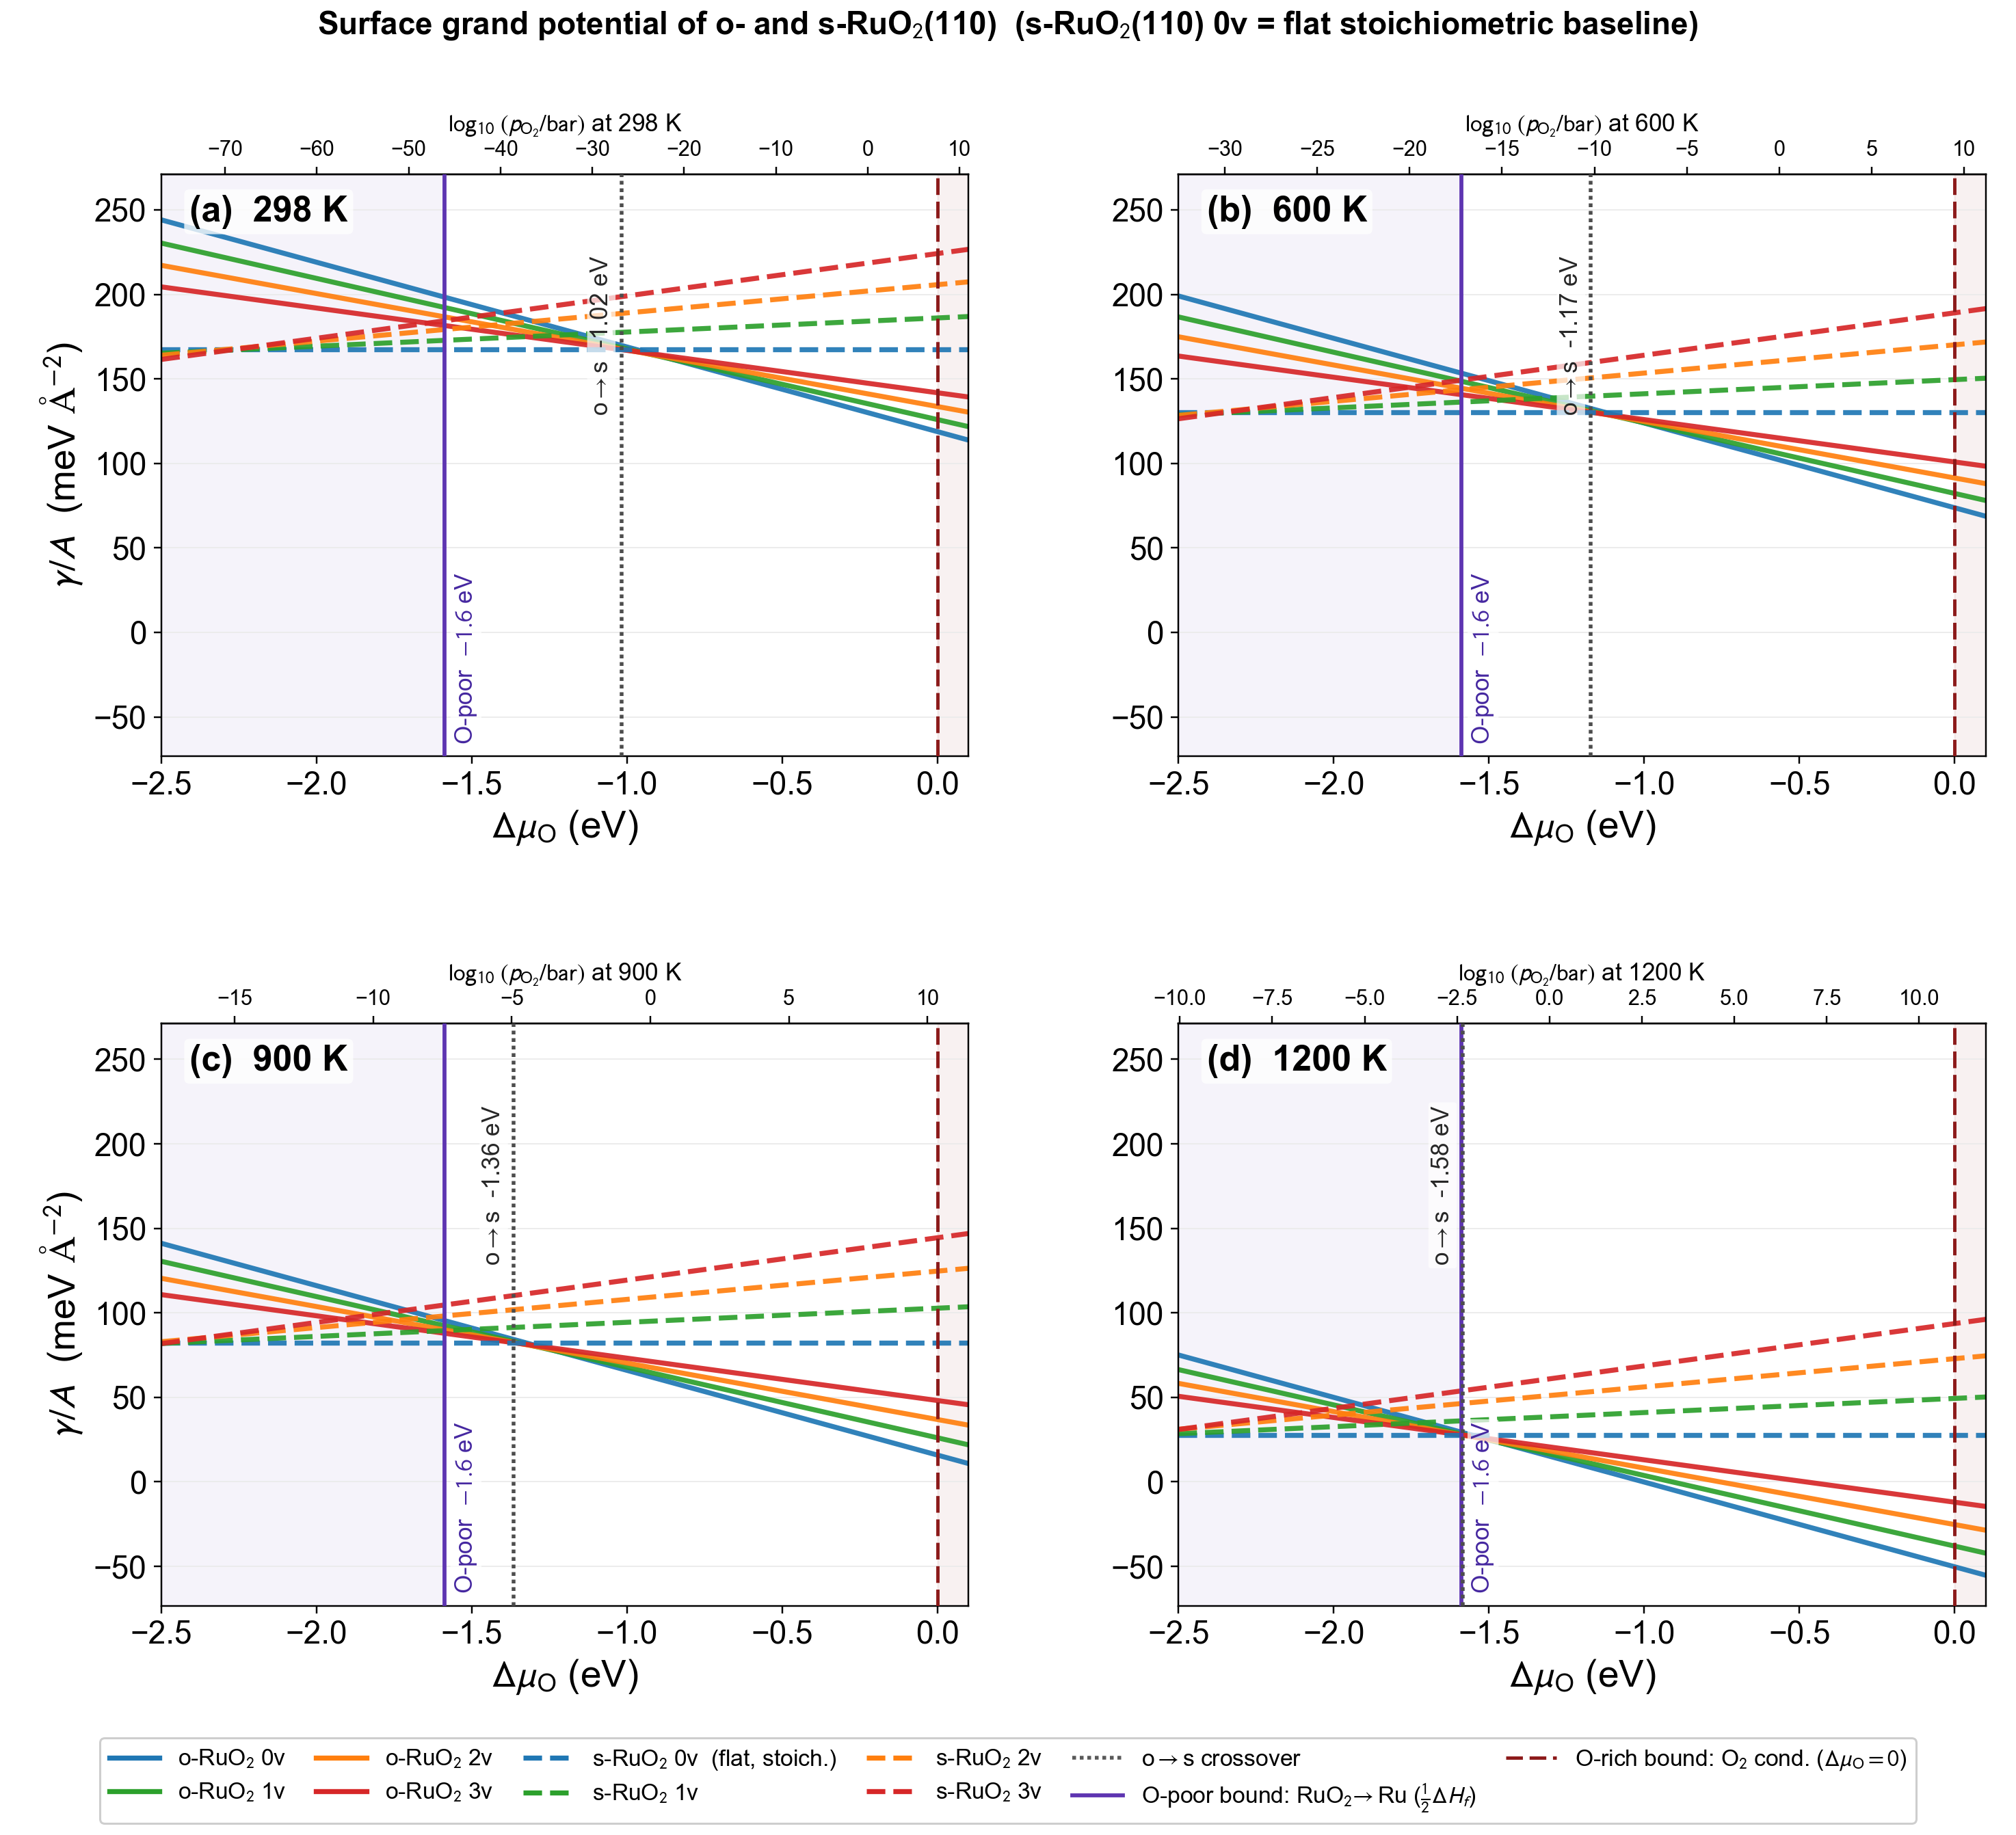
\includegraphics[width=\linewidth]{fig_bulk_referenced_2x2_dft.png}
  \caption{Surface grand potential of the \textit{o}- and
  \textit{s}-RuO$_2$(110) terminations referenced to bulk RuO$_2$ (absolute
  surface free energy $\gamma$) at (a)~298, (b)~600, (c)~900 and (d)~1200~K.
  Solid lines, \textit{o}-RuO$_2$(110) $k$-vacancy surfaces; dashed lines,
  \textit{s}-RuO$_2$(110); the stoichiometric \textit{s}-RuO$_2$(110) 0v surface
  is flat. The dotted line marks the \textit{o}$\rightarrow$\textit{s} boundary
  separating stable \textit{s}-RuO$_2$(110) (left) from \textit{o}-RuO$_2$(110)
  (right), identical to that of Figure~\ref{fig:unified}. Shaded bands are
  thermodynamically
  inaccessible: the oxygen-rich limit at $\Delta\mu_{\mathrm O}=0$ (O$_2$
  condensation) and the oxygen-poor limit at
  $\Delta\mu_{\mathrm O}=\tfrac{1}{2}\Delta H_f^{\,\mathrm{RuO_2}}\approx-1.60$~eV
  (decomposition to metallic Ru, Eq.~\eqref{eq:opoor}). The upper axis of each
  panel gives the corresponding oxygen partial pressure,
  $\log_{10}\!\left(p_{\mathrm{O_2}}/\mathrm{bar}\right)$, at that temperature
  (Eq.~\eqref{eq:pO2}). All panels share a common $\gamma$ axis.}
  \label{fig:bulkref}
\end{figure*}
